\documentclass[12pt]{article}
\usepackage{fontspec}
\usepackage{fullpage}
\usepackage{hyperref}
\hypersetup{bookmarks=true,colorlinks=true,linkcolor=red,citecolor=blue,filecolor=magenta,urlcolor=cyan}
\usepackage{amsmath}
\usepackage{amssymb}
\usepackage{mathtools}
\usepackage{unicode-math}
\usepackage{tabu}
\usepackage{longtable}
\usepackage{booktabs}
\usepackage{caption}
\usepackage{graphics}
\usepackage{filecontents}
\usepackage[backend=bibtex]{biblatex}
\usepackage{url}
\setmathfont{Latin Modern Math}
\global\tabulinesep=1mm
\newcounter{assumpnum}
\newcommand{\atheassumpnum}{A\theassumpnum}
\newcounter{lcnum}
\newcommand{\lcthelcnum}{LC\thelcnum}
\newcounter{ucnum}
\newcommand{\uctheucnum}{UC\theucnum}
\bibliography{bibfile}
\title{Software Requirements Specification for Slope Stability Analysis}
\author{HenryFrankis}
\begin{document}
\maketitle
\tableofcontents
\newpage
\section{Reference Material}
\label{Sec:RefMat}
This section records information for easy reference.
\subsection{Table of Units}
\label{Sec:ToU}
The unit system used throughout is SI (Système International d'Unités). In addition to the basic units, several derived units are also used. For each unit, the table lists the symbol, a description and the SI name.
\begin{longtable*}{l l}
\toprule
Symbol & Description
\\
\midrule
${}^{\circ}$ & angle (degree)
\\
m & length (metre)
\\
N & force (newton)
\\
Pa & pressure (pascal)
\\
\bottomrule
\label{Table:ToU}
\end{longtable*}
\subsection{Table of Symbols}
\label{Sec:ToS}
The table that follows summarizes the symbols used in this document along with their units. Throughout the document, values with a subscript $i$ implies that the value will be taken at and analyzed at a slice or slice interface composing the total slip mass.
\begin{longtabu}{l X[l] l}
\toprule
Symbol & Description & Units
\\
\midrule
$\{{x_{cs}}{,y_{cs}}\}$ & The Set of X and Y Coordinates: describe the vertices of the critical slip surface & m
\\
$(x,y)$ & Cartesian Position Coordinates: y is considered parallel to the direction of the force of gravity and x is considered perpendicular to y & m
\\
$a$ & Constant: FIXME: missing description & m
\\
$A$ & Constant: FIXME: missing description & m
\\
$b$ & Base Width of a Slice: in the x-ordinate direction only for slice index i & m
\\
$c'$ & Effective Cohesion: internal pressure that sticks particles of soil together & Pa
\\
${C1_{i}}$ & Interslice Normal Force Function: the normal force at the interslice interface for slice i & Nm
\\
${C2_{i}}$ & Interslice Shear Force Function: the shear force at the interslice interface for slice i & Nm
\\
$E$ & Elastic Modulus: The ratio of the stress exerted on a body to the resulting strain. & Pa
\\
$F$ & Force: An interaction that tends to produce change in the motion of an object & N
\\
${F_{x}}$ & X-Component of the Net Force:  & N
\\
${F_{y}}$ & Y-Component of the Net Force:  & N
\\
$f$ & Scaling Function: magnitude of interslice forces as a function of the x coordinatefor interslice index i; can be constant or a half-sine & 
\\
$FS$ & Factor of Safety: The global stability of a surface in a slope & 
\\
${FS_{Loc,i}}$ & Local Factor of Safety: for slice index i & 
\\
${FS_{min}}$ & Minimum Factor of Safety: The minimum factor of safety & 
\\
$G$ & Interslice Normal Force: exerted between adjacent slices for interslice index i & N
\\
$H$ & Interslice Water Force: exerted in the x-ordinate direction between adjacent slices for interslice index i & N
\\
$ΔH$ & Difference Between Interslice Forces: exerted in the x-ordinate direction between adjacent slices for interslice index i & N
\\
$h$ & Midpoint Height: distance from the slip base to the slope surface in a vertical line from the midpoint of the slice for slice index i & m
\\
$i$ & Index: used to show a quantity applies to only one slice & 
\\
${K_{bA}}$ & Effective Base Stiffness a: for rotated coordinates of a slice base surface, for slice index i & $\frac{\text{Pa}}{\text{m}}$
\\
${K_{bB}}$ & Effective Base Stiffness a: for rotated coordinates of a slice base surface, for slice index i & $\frac{\text{Pa}}{\text{m}}$
\\
$K$ & Stiffness: The extent a body resists strain. & $\frac{\text{N}}{\text{m}}$
\\
${K_{bn}}$ & Normal Stiffness: for a slice base surface, without length adjustment for slice index i & $\frac{\text{Pa}}{\text{m}}$
\\
${K_{bt}}$ & Shear Stiffness: for a slice base surface, without length adjustment for slice index i & $\frac{\text{Pa}}{\text{m}}$
\\
${K_{c}}$ & Earthquake Load Factor: proportionality factor of force that weight pushes outwards; caused by seismic earth movements & 
\\
${K_{no}}$ & Normal Stiffness: residual strength & $\frac{\text{Pa}}{\text{m}}$
\\
${K_{sn}}$ & Normal Stiffness: for an interslice surface, without length adjustment for interslice index i & $\frac{\text{Pa}}{\text{m}}$
\\
${K_{st}}$ & Shear Stiffness: for interslice surface, without length adjustment for interslice index i & $\frac{\text{Pa}}{\text{m}}$
\\
${K_{tr}}$ & Shear Stiffness: residual strength & $\frac{\text{Pa}}{\text{m}}$
\\
$M$ & Moment: a measure of the tendency of a body to rotate about a specific point or axis & Nm
\\
$N$ & Normal Force: total reactive force for a soil surface subject to a body resting on it & N
\\
$N'$ & Effective Normal Force: for a soil surface, subtracting pore water reactive force from total reactive force & N
\\
$n$ & Number of Slices: the slip mass has been divided into & 
\\
$N*$ & Effective Normal Force: for a soil surface, without the influence of interslice forces & N
\\
$p$ & Pressure: A force exerted over an area & Pa
\\
$P$ & Resistive Shear Force: Mohr Coulomb frictional force that describes the limit of mobilized shear force the slice i can withstand before failure & N
\\
$Q$ & Imposed Surface Load: a downward force acting into the surface from midpoint of slice i & N
\\
$R$ & Resistive Shear Force: without the influence of interslice forces for slice index i & N
\\
$S$ & Mobilized Shear Force: for slice index i & N
\\
$s$ & Mobilized Shear Stress: acting on the base of a slice & Pa
\\
$SpencerFixme1Please$ & Fixme: What is this value? & 
\\
$SpencerFixme2Please$ & Fixme: What is this value? & 
\\
$T$ & Mobilized Shear Force: without the influence of interslice forces for slice index i & N
\\
${U_{b}}$ & Base Hydrostatic Force: from water pressure within the slice for slice index i & N
\\
${U_{t}}$ & Surface Hydrostatic Force: from water pressure acting into the slice from standing water on the slope surface for slice index i & N
\\
$u$ & Local Index: used as a bound variable index in calculations & 
\\
$v$ & Local Index: used as a bound variable index in calculations & 
\\
$W$ & Weight: downward force caused by gravity on slice i & N
\\
$x$ & X Ordinate: refers to either slice i midpoint, or slice interface i & m
\\
${x_{slip}}$ & X Ordinate: distance of the slip surface at i, refers to either slice i midpoint, or slice interface i & m
\\
${x_{us}}$ & X Ordinate: distance of the edge of the slope at i, refers to either slice i midpoint, or slice interface i & m
\\
$X$ & Interslice Shear Force: exerted between adjacent slices for interslice index i & N
\\
${y_{slip}}$ & Y Ordinate: height of the slip surface at i, refers to either slice i midpoint, or slice interface i & m
\\
${y_{us}}$ & Y Ordinate: height of the top of the slope at i, refers to either slice i midpoint, or slice interface i & m
\\
${y_{wt}}$ & Y Ordinate: height of the water table at i, refers to either slice i midpoint, or slice interface i & m
\\
$y$ & Y Ordinate: refers to either slice i midpoint, or slice interface i & m
\\
$z$ & Center of Slice Height: the distance from the lowest part of the slice to the height of the centers of slice & m
\\
$α$ & Angle: base of the mass relative to the horizontal for slice index i & ${}^{\circ}$
\\
$β$ & Angle: surface of the mass relative to the horizontal for slice index i & ${}^{\circ}$
\\
$γ$ & Dry Unit Weight: The weight of a dry soil/ground layer divided by the volume of the layer. & $\frac{\text{N}}{\text{m}^{3}}$
\\
${γ_{Sat}}$ & Saturated Unit Weight: The weight of saturated soil/ground layer divided by the volume of the layer. & $\frac{\text{N}}{\text{m}^{3}}$
\\
${γ_{w}}$ & Unit Weight of Water: The weight of one cubic meter of water. & $\frac{\text{N}}{\text{m}^{3}}$
\\
$δ$ & Displacement: generic displacement of a body & m
\\
$δn$ & Displacement: for the element parallel to the surface for slice index i & m
\\
$δt$ & Displacement: for the element normal to the surface for slice index i & m
\\
$δu$ & Displacement: shear displacement for slice index i & m
\\
$δv$ & Displacement: normal displacement for slice index i & m
\\
$δx$ & Displacement: in the x-ordinate direction for slice index i & m
\\
$δy$ & Displacement: in the y-ordinate direction for slice index i & m
\\
$ε$ & Displacement: in rotated coordinate system & m
\\
$κ$ & Constant: FIXME: missing description & Pa
\\
$λ$ & Interslice Normal/shear Force Ratio: applied to all interslices & 
\\
$μ$ & Pore Pressure: from water within the soil & Pa
\\
$ν$ & Poisson's Ratio: The ratio of perpendicular strain to parallel strain. & 
\\
$σ$ & Normal Stress: The stress exerted perpendicular to the plane of the object & Pa
\\
$τ$ & Resistive Shear Stress: acting on the base of a slice & Pa
\\
$Υ$ & Function: generic minimization function or algorithm & 
\\
$φ'$ & Effective Angle of Friction: The angle of inclination with respect to the horizontal axis of the Mohr-Coulomb shear resistance line & ${}^{\circ}$
\\
$Φ$ & Constant: converts resistive shear without the influence of interslice forces, to a calculation considering the interslice forces & N
\\
$Ψ$ & Constant: converts mobile shear without the influence of interslice forces, to a calculation considering the interslice forces & N
\\
$ω$ & Angle: of imposed surface load acting into the surface relative to the vertical for slice index i & ${}^{\circ}$
\\
${ℓ_{b}}$ & Total Base Length of a Slice: for slice index i & m
\\
${ℓ_{s}}$ & Length of an Interslice Surface: from slip base to slope surface in a vertical line from an interslice vertex for interslice index i & m
\\
\bottomrule
\label{Table:ToS}
\end{longtabu}
\subsection{Abbreviations and Acronyms}
\label{Sec:TAbbAcc}
\begin{longtable*}{l l}
\toprule
Symbol & Description
\\
\midrule
A & Assumption
\\
DD & Data Definition
\\
GD & General Definition
\\
GS & Goal Statement
\\
IM & Instance Model
\\
LC & Likely Change
\\
PS & Physical System Description
\\
R & Requirement
\\
SRS & Software Requirements Specification
\\
SSA & Slope Stability Analysis
\\
T & Theoretical Model
\\
TU & Typical Uncertainty
\\
UC & Unlikely Change
\\
\bottomrule
\label{Table:TAbbAcc}
\end{longtable*}
\section{Introduction}
\label{Sec:Intro}
A slope of geological mass, composed of soil and rock, is subject to the influence of gravity on the mass. For an unstable slope this can cause instability in the form of soil/rock movement. The effects of soil/rock movement can range from inconvenient to seriously hazardous, resulting in signifcant life and economic losses. Slope stability is of interest both when analyzing natural slopes, and when designing an excavated slope. Slope stability analysis is the assessment of the safety of a slope, identifying the surface most likely to experience slip and an index of its relative stability known as the factor of safety.
The following section provides an overview of the Software Requirements Specification (SRS) for a slope stability analysis problem. The developed program will be referred to as the Slope Stability Analysis (SSA) program. This section explains the purpose of this document, the scope of the system, the organization of the document, and the characteristics of the intended reader.
\subsection{Purpose of Document}
\label{Sec:DocPurpose}
The SSA program determines the critical slip surface, and its respective factor of safety as a method of assessing the stability of a slope design. The program is intended to be used as an educational tool for introducing slope stability issues, and will facilitate the analysis and design of a safe slope.
This document will be used as a starting point for subsequent development phases, including writing the design specification and the software verification and validation plan. The design document will show how the requirements are to be realized, including decisions on the numerical algorithms and programming environment. The verification and validation plan will show the steps that will be used to increase confidence in the software documentation and the implementation. Although the SRS fits in a series of documents that follow the so-called waterfall model, the actual development process is not constrained in any way. Even when the waterfall model is not followed, as Parnas and Clements point out \cite{parnasClements1986}, the most logical way to present the documentation is still to ``fake'' a rational design process.
\subsection{Scope of Requirements}
\label{Sec:ReqsScope}
The scope of the requirements includes stability analysis of a 2 dimensional slope, composed of homogeneous soil layers. Given the appropriate inputs, the code for SSA is intended to identify the most likely failure surface within the possible input range, and find the factor of safety for the slope as well as displacement of soil that will occur on the slope.
\subsection{Characteristics of Intended Reader}
\label{Sec:ReaderChars}
Reviewers of this documentation should have a strong knowledge in solid mechanics. The reviewers should also have an understanding of undergraduate level 4 physics. The users of SSA can have a lower level of expertise, as explained in Section~\ref{Sec:UserChars}.
\subsection{Organization of Document}
\label{Sec:DocOrg}
The organization of this document follows the template for an SRS for scientific computing software proposed by Koothoor as well as Smith and Lai. The presentation follows the standard pattern of presenting goals, theories, definitions, and assumptions. For readers that would like a more bottom up approach, they can start reading the instance models in Section~\ref{Sec:IMs} and trace back to find any additional information they require.
The goal statements are refined to the theoretical models, and the theoretical models to the instance models. The instance models provide the set of algebraic equations that must be solved iteratively to perform a Morgenstern Price Analysis.
\section{General System Description}
\label{Sec:GenSysDesc}
This section provides general information about the system including identifying the interfaces between the system and its environment (system context), describing the user characteristics and listing the system constraints.
\subsection{User Characteristics}
\label{Sec:UserChars}
The end user of SSA should have an understanding of undergraduate Level 1 Calculus and Physics, and be familiar with soil and material properties.
\subsection{System Constraints}
\label{Sec:SysConstraints}
There are no system constraints.
\section{Specific System Description}
\label{Sec:SpecSystDesc}
This section first presents the problem description, which gives a high-level view of the problem to be solved. This is followed by the solution characteristics specification, which presents the assumptions, theories, definitions and finally the instance models that model the slope.
\subsection{Problem Description}
\label{Sec:ProbDesc}
SSA is a computer program developed to evaluate the factor of safety of a slope's slip surface and to calculate the displacement that the slope will experience.
\subsubsection{Terminology and Definitions}
\label{Sec:TermDefs}
This subsection provides a list of terms that are used in the subsequent sections and their meaning, with the purpose of reducing ambiguity and making it easier to correctly understand the requirements.
\begin{itemize}
\item[Factor of Safety:]The global stability of a surface in a slope
\item[Critical Slip Surface:]Slip surface of the slope that has the lowest global factor of safety, and therefore most likely to experience failure.
\item[Stress:]Forces that are exerted between planes internal to a larger body subject to external loading.
\item[Strain:]Stress forces that result in deformation of the body/plane.
\item[Normal Force:]A force applied perpendicular to the plane of the material.
\item[Shear Force:]A force applied parallel to the plane of the material.
\item[Tension:]A stress that causes displacement of the body away from its center.
\item[Compression:]A stress that causes displacement of the body towards its center.
\item[Plane Strain:]The resultant stresses in one of the directions of a 3 dimensional material can be approximated as 0. Results when the length of one dimension of the body dominates the others. Stresses in the dominant dimensions direction are the ones that can be approximated as 0.
\end{itemize}
\subsubsection{Physical System Description}
\label{Sec:PhysSyst}
Analysis of the slope is performed by looking at properties of the slope as a series of slice elements. Some properties are interslice properties, and some are slice or slice base properties. The index convention for referencing which interslice or slice is being used is shown in Figure~\ref{Figure:IndexConvention}.
\begin{itemize}
\item{Interslice properties convention is noted by j. The end interslice properties are usually not of interest, therefore use the interslice properties from $1\leq{}i\leq{}n-1$.}
\item{Slice properties convention is noted by $i$.}
\end{itemize}
A free body diagram of the forces acting on the slice is displayed in Figure~\ref{Figure:ForceDiagram}.
\begin{figure}
\begin{center}
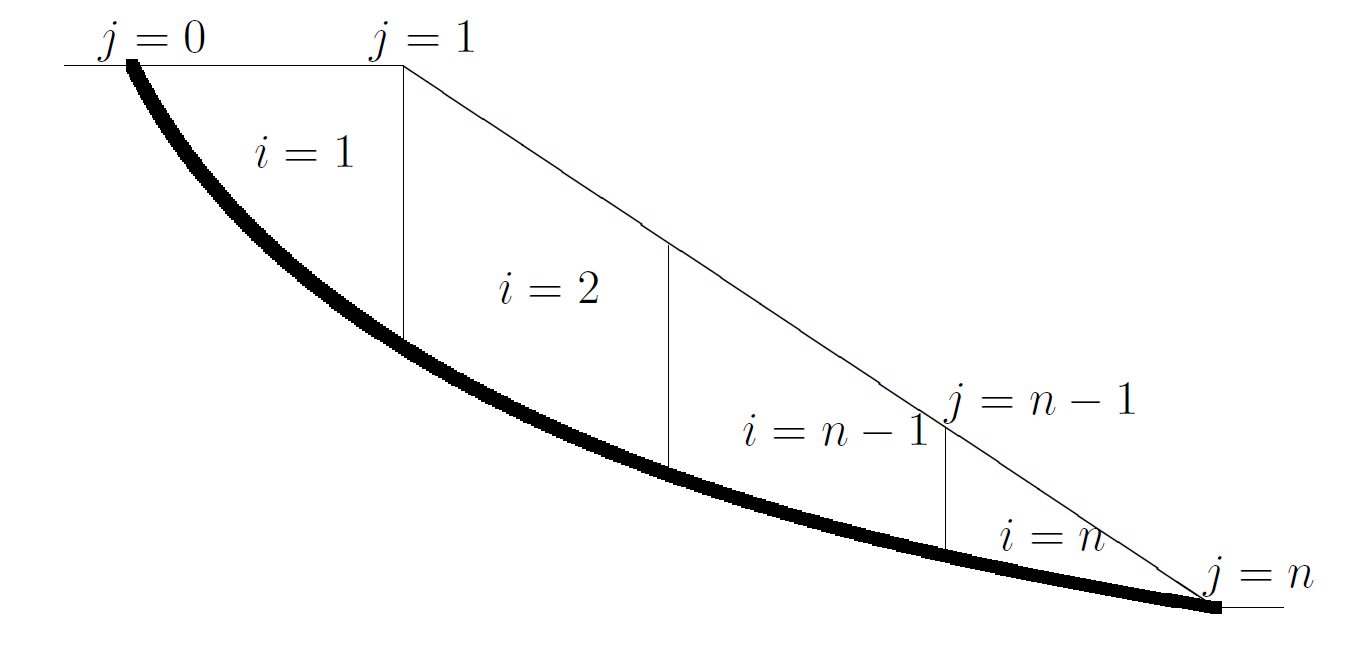
\includegraphics[width=\textwidth]{../../../datafiles/SSP/IndexConvention.png}
\caption{Index convention for numbering slice and interslice force variables}
\label{Figure:IndexConvention}
\end{center}
\end{figure}
\begin{figure}
\begin{center}
\includegraphics[width=\textwidth]{../../../datafiles/SSP/ForceDiagram.png}
\caption{Forces acting on a slice}
\label{Figure:ForceDiagram}
\end{center}
\end{figure}
\subsubsection{Goal Statements}
\label{Sec:GoalStmt}
Given the geometry of the water table, the geometry of the layers composing the plane of a slope, and the material properties of the layers, the goal statements are:
\begin{itemize}
\item[GS1:]Evaluate local and global factors of safety along a given slip surface.
\item[GS2:]Identify the critical slip surface for the slope, with the lowest factor of safety.
\item[GS3:]Determine the displacement of the slope.
\end{itemize}
\subsection{Solution Characteristics Specification}
\label{Sec:SolCharSpec}
The instance models that govern SSA are presented in Section~\ref{Sec:IMs}. The information to understand the meaning of the instance models and their derivation is also presented, so that the instance models can be verified.
\subsubsection{Assumptions}
\label{Sec:Assumps}
This section simplifies the original problem and helps in developing the theoretical model by filling in the missing information for the physical system. The numbers given in the square brackets refer to the Theoretical Models {[}Section~\ref{Sec:TMs}{]}, General Definitions {[}Section~\ref{Sec:GDs}{]}, Data Definitions {[}Section~\ref{Sec:DDs}{]}, Instance Models {[}Section~\ref{Sec:IMs}{]}, Likely Changes {[}Section~\ref{Sec:LCs}{]}, or Unlikely Changes {[}Section~\ref{Sec:UCs}{]}, in which the respective assumption is used.
\begin{description}
\item[\refstepcounter{assumpnum}\atheassumpnum\label{A:Slip-Surface-Concave}:]The slip surface is concave with respect to the slope surface. The $(x,y)$ coordinates of the failure surface follow a monotonic function.
\end{description}
\begin{description}
\item[\refstepcounter{assumpnum}\atheassumpnum\label{A:Geo-Slope-Mat-Props-of-Soil-Inputs}:]The geometry of the slope, and the material properties of the soil layers are given as inputs.
\end{description}
\begin{description}
\item[\refstepcounter{assumpnum}\atheassumpnum\label{A:Soil-Layer-Homogeneous}:]The different layers of the soil are homogeneous, with consistent soil properties throughout, and independent of dry or saturated conditions, with the exception of unit weight.
\end{description}
\begin{description}
\item[\refstepcounter{assumpnum}\atheassumpnum\label{A:Soil-Layers-Isotropic}:]Soil layers are treated as if they have isotropic properties.
\end{description}
\begin{description}
\item[\refstepcounter{assumpnum}\atheassumpnum\label{A:Interslice-Norm-Shear-Forces-Linear}:]Interslice normal and shear forces have a linear relationship, proportional to a constant ($λ$) and an interslice force function ($f$) depending on x position.
\end{description}
\begin{description}
\item[\refstepcounter{assumpnum}\atheassumpnum\label{A:Base-Norm-Shear-Forces-Linear-on-FS}:]Slice to base normal and shear forces have a linear relationship, dependent on the factor of safety $FS$, and the Coulomb sliding law.
\end{description}
\begin{description}
\item[\refstepcounter{assumpnum}\atheassumpnum\label{A:Stress-Strain-Curve-interslice-Linear}:]The stress - strain curve for interslice relationships is linear with a constant slope.
\end{description}
\begin{description}
\item[\refstepcounter{assumpnum}\atheassumpnum\label{A:Plane-Strain-Conditions}:]The slope and slip surface extends far into and out of the geometry (z coordinate). This implies plane strain conditions, making 2D analysis appropriate.
\end{description}
\begin{description}
\item[\refstepcounter{assumpnum}\atheassumpnum\label{A:Effective-Norm-Stress-Large}:]The effective normal stress is large enough that the resistive shear to effective normal stress relationship can be approximated as a linear relationship.
\end{description}
\begin{description}
\item[\refstepcounter{assumpnum}\atheassumpnum\label{A:Surface-Base-Slice-between-Interslice-Straight-Lines}:]The surface and base of a slice between interslice nodes are approximated as straight lines.
\end{description}
\subsubsection{Theoretical Models}
\label{Sec:TMs}
This section focuses on the general equations and laws that SSA is based on.
~\newline
\noindent \begin{minipage}{\textwidth}
\begin{tabular}{p{0.2\textwidth} p{0.73\textwidth}}
\toprule \textbf{Refname} & \textbf{T:fs.rc}
\phantomsection 
\label{T:fs.rc}
\\ \midrule \\
Label & Factor of safety
\\ \midrule \\
Equation & \begin{dmath}
           FS=\frac{P}{S}
           \end{dmath}
\\ \midrule \\
Description & \begin{symbDescription}
              \item{$FS$ is the factor of safety (Unitless)}
              \item{$P$ is the resistive shear force (N)}
              \item{$S$ is the mobilized shear force (N)}
              \end{symbDescription}
\\ \midrule \\
Source & FIXME: This needs to be filled in
\\ \midrule \\
RefBy & FIXME: This needs to be filled in
\\ \bottomrule \end{tabular}
\end{minipage}\\
~\newline
\noindent \begin{minipage}{\textwidth}
\begin{tabular}{p{0.2\textwidth} p{0.73\textwidth}}
\toprule \textbf{Refname} & \textbf{T:equilibrium}
\phantomsection 
\label{T:equilibrium}
\\ \midrule \\
Label & Equilibrium
\\ \midrule \\
Equation & \begin{dmath}
           \displaystyle\sum{{F_{x}}}=\displaystyle\sum{{F_{y}}}=\displaystyle\sum{M}=0
           \end{dmath}
\\ \midrule \\
Description & \begin{symbDescription}
              \item{${F_{x}}$ is the x-component of the net force (N)}
              \item{${F_{y}}$ is the y-component of the net force (N)}
              \item{$M$ is the moment (Nm)}
              \end{symbDescription}
\\ \midrule \\
Source & FIXME: This needs to be filled in
\\ \midrule \\
RefBy & FIXME: This needs to be filled in
\\ \bottomrule \end{tabular}
\end{minipage}\\
~\newline
\noindent \begin{minipage}{\textwidth}
\begin{tabular}{p{0.2\textwidth} p{0.73\textwidth}}
\toprule \textbf{Refname} & \textbf{T:mcShrStrgth}
\phantomsection 
\label{T:mcShrStrgth}
\\ \midrule \\
Label & Mohr-Coulumb shear strength
\\ \midrule \\
Equation & \begin{dmath}
           τ=σ \tan\left(φ'\right)+c'
           \end{dmath}
\\ \midrule \\
Description & \begin{symbDescription}
              \item{$τ$ is the resistive shear stress (Pa)}
              \item{$σ$ is the normal stress (Pa)}
              \item{$φ'$ is the effective angle of friction (${}^{\circ}$)}
              \item{$c'$ is the effective cohesion (Pa)}
              \end{symbDescription}
\\ \midrule \\
Source & FIXME: This needs to be filled in
\\ \midrule \\
RefBy & FIXME: This needs to be filled in
\\ \bottomrule \end{tabular}
\end{minipage}\\
~\newline
\noindent \begin{minipage}{\textwidth}
\begin{tabular}{p{0.2\textwidth} p{0.73\textwidth}}
\toprule \textbf{Refname} & \textbf{T:effStress}
\phantomsection 
\label{T:effStress}
\\ \midrule \\
Label & Effective stress
\\ \midrule \\
Equation & \begin{dmath}
           σ=σ-μ
           \end{dmath}
\\ \midrule \\
Description & \begin{symbDescription}
              \item{$σ$ is the normal stress (Pa)}
              \item{$μ$ is the pore pressure (Pa)}
              \end{symbDescription}
\\ \midrule \\
Source & FIXME: This needs to be filled in
\\ \midrule \\
RefBy & FIXME: This needs to be filled in
\\ \bottomrule \end{tabular}
\end{minipage}\\
~\newline
\noindent \begin{minipage}{\textwidth}
\begin{tabular}{p{0.2\textwidth} p{0.73\textwidth}}
\toprule \textbf{Refname} & \textbf{T:hookesLaw}
\phantomsection 
\label{T:hookesLaw}
\\ \midrule \\
Label & Hooke's law
\\ \midrule \\
Equation & \begin{dmath}
           F=K δ
           \end{dmath}
\\ \midrule \\
Description & \begin{symbDescription}
              \item{$F$ is the force (N)}
              \item{$K$ is the stiffness ($\frac{\text{N}}{\text{m}}$)}
              \item{$δ$ is the displacement (m)}
              \end{symbDescription}
\\ \midrule \\
Source & FIXME: This needs to be filled in
\\ \midrule \\
RefBy & FIXME: This needs to be filled in
\\ \bottomrule \end{tabular}
\end{minipage}\\
\subsubsection{General Definitions}
\label{Sec:GDs}
This section collects the laws and equations that will be used in deriving the data definitions, which in turn are used to build the instance models.
~\newline
\noindent \begin{minipage}{\textwidth}
\begin{tabular}{p{0.2\textwidth} p{0.73\textwidth}}
\toprule \textbf{Refname} & \textbf{GD:normForcEq}
\phantomsection 
\label{GD:normForcEq}
\\ \midrule \\
Label & Normal force equilibrium
\\ \midrule \\
Equation & \begin{dmath}
           N_{i}=\left(W_{i}-X_{i-1}+X_{i}+{U_{t,i}} \cos\left(β_{i}\right)+Q_{i} \cos\left(ω_{i}\right)\right) \cos\left(α_{i}\right)+\left(-{K_{c}} W_{i}-G_{i}+G_{i-1}-H_{i}+H_{i-1}+{U_{t,i}} \sin\left(β_{i}\right)+Q_{i} \sin\left(ω_{i}\right)\right) \sin\left(α_{i}\right)
           \end{dmath}
\\ \midrule \\
Description & \begin{symbDescription}
              \item{$N$ is the normal force (N)}
              \item{$i$ is the index (Unitless)}
              \item{$W$ is the weight (N)}
              \item{$X$ is the interslice shear force (N)}
              \item{${U_{t}}$ is the surface hydrostatic force (N)}
              \item{$β$ is the angle (${}^{\circ}$)}
              \item{$Q$ is the imposed surface load (N)}
              \item{$ω$ is the angle (${}^{\circ}$)}
              \item{$α$ is the angle (${}^{\circ}$)}
              \item{${K_{c}}$ is the earthquake load factor (Unitless)}
              \item{$G$ is the interslice normal force (N)}
              \item{$H$ is the interslice water force (N)}
              \end{symbDescription}
\\ \midrule \\
Source &
\\ \midrule \\
RefBy & FIXME: This needs to be filled in
\\ \bottomrule \end{tabular}
\end{minipage}\\
~\newline
\noindent \begin{minipage}{\textwidth}
\begin{tabular}{p{0.2\textwidth} p{0.73\textwidth}}
\toprule \textbf{Refname} & \textbf{GD:bsShrFEq}
\phantomsection 
\label{GD:bsShrFEq}
\\ \midrule \\
Label & Base shear force equilibrium
\\ \midrule \\
Equation & \begin{dmath}
           S_{i}=\left(W_{i}-X_{i-1}+X_{i}+{U_{t,i}} \cos\left(β_{i}\right)+Q_{i} \cos\left(ω_{i}\right)\right) \sin\left(α_{i}\right)+\left(-{K_{c}} W_{i}-G_{i}+G_{i-1}-H_{i}+H_{i-1}+{U_{t,i}} \sin\left(β_{i}\right)+Q_{i} \sin\left(ω_{i}\right)\right) \cos\left(α_{i}\right)
           \end{dmath}
\\ \midrule \\
Description & \begin{symbDescription}
              \item{$S$ is the mobilized shear force (N)}
              \item{$i$ is the index (Unitless)}
              \item{$W$ is the weight (N)}
              \item{$X$ is the interslice shear force (N)}
              \item{${U_{t}}$ is the surface hydrostatic force (N)}
              \item{$β$ is the angle (${}^{\circ}$)}
              \item{$Q$ is the imposed surface load (N)}
              \item{$ω$ is the angle (${}^{\circ}$)}
              \item{$α$ is the angle (${}^{\circ}$)}
              \item{${K_{c}}$ is the earthquake load factor (Unitless)}
              \item{$G$ is the interslice normal force (N)}
              \item{$H$ is the interslice water force (N)}
              \end{symbDescription}
\\ \midrule \\
Source &
\\ \midrule \\
RefBy & FIXME: This needs to be filled in
\\ \bottomrule \end{tabular}
\end{minipage}\\
~\newline
\noindent \begin{minipage}{\textwidth}
\begin{tabular}{p{0.2\textwidth} p{0.73\textwidth}}
\toprule \textbf{Refname} & \textbf{GD:resShr}
\phantomsection 
\label{GD:resShr}
\\ \midrule \\
Label & Resistive shear force
\\ \midrule \\
Equation & \begin{dmath}
           P_{i}={N'}_{i} \tan\left({φ'}_{i}\right)+{c'}_{i} b_{i} \sec\left(α_{i}\right)
           \end{dmath}
\\ \midrule \\
Description & \begin{symbDescription}
              \item{$P$ is the resistive shear force (N)}
              \item{$i$ is the index (Unitless)}
              \item{$N'$ is the effective normal force (N)}
              \item{$φ'$ is the effective angle of friction (${}^{\circ}$)}
              \item{$c'$ is the effective cohesion (Pa)}
              \item{$b$ is the base width of a slice (m)}
              \item{$α$ is the angle (${}^{\circ}$)}
              \end{symbDescription}
\\ \midrule \\
Source &
\\ \midrule \\
RefBy & FIXME: This needs to be filled in
\\ \bottomrule \end{tabular}
\end{minipage}\\
~\newline
\noindent \begin{minipage}{\textwidth}
\begin{tabular}{p{0.2\textwidth} p{0.73\textwidth}}
\toprule \textbf{Refname} & \textbf{GD:mobShr}
\phantomsection 
\label{GD:mobShr}
\\ \midrule \\
Label & Mobile shear force
\\ \midrule \\
Equation & \begin{dmath}
           S_{i}=\frac{P_{i}}{FS}=\frac{{N'}_{i} \tan\left({φ'}_{i}\right)+{c'}_{i} b_{i} \sec\left(α_{i}\right)}{FS}
           \end{dmath}
\\ \midrule \\
Description & \begin{symbDescription}
              \item{$S$ is the mobilized shear force (N)}
              \item{$i$ is the index (Unitless)}
              \item{$P$ is the resistive shear force (N)}
              \item{$FS$ is the factor of safety (Unitless)}
              \item{$N'$ is the effective normal force (N)}
              \item{$φ'$ is the effective angle of friction (${}^{\circ}$)}
              \item{$c'$ is the effective cohesion (Pa)}
              \item{$b$ is the base width of a slice (m)}
              \item{$α$ is the angle (${}^{\circ}$)}
              \end{symbDescription}
\\ \midrule \\
Source &
\\ \midrule \\
RefBy & FIXME: This needs to be filled in
\\ \bottomrule \end{tabular}
\end{minipage}\\
~\newline
\noindent \begin{minipage}{\textwidth}
\begin{tabular}{p{0.2\textwidth} p{0.73\textwidth}}
\toprule \textbf{Refname} & \textbf{GD:normShrR}
\phantomsection 
\label{GD:normShrR}
\\ \midrule \\
Label & Interslice normal/shear relationship
\\ \midrule \\
Equation & \begin{dmath}
           X=λ f G
           \end{dmath}
\\ \midrule \\
Description & \begin{symbDescription}
              \item{$X$ is the interslice shear force (N)}
              \item{$λ$ is the interslice normal/shear force ratio (Unitless)}
              \item{$f$ is the scaling function (Unitless)}
              \item{$G$ is the interslice normal force (N)}
              \end{symbDescription}
\\ \midrule \\
Source &
\\ \midrule \\
RefBy & FIXME: This needs to be filled in
\\ \bottomrule \end{tabular}
\end{minipage}\\
~\newline
\noindent \begin{minipage}{\textwidth}
\begin{tabular}{p{0.2\textwidth} p{0.73\textwidth}}
\toprule \textbf{Refname} & \textbf{GD:momentEql}
\phantomsection 
\label{GD:momentEql}
\\ \midrule \\
Label & Moment equilibrium
\\ \midrule \\
Equation & \begin{dmath}
           0=-G_{i} \left(z_{i}-\frac{b_{i}}{2} \tan\left(α_{i}\right)\right)+G_{i-1} \left(z_{i-1}-\frac{b_{i}}{2} \tan\left(α_{i}\right)\right)-H_{i} \left(z_{i}-\frac{b_{i}}{2} \tan\left(α_{i}\right)\right)+H_{i-1} \left(z_{i-1}-\frac{b_{i}}{2} \tan\left(α_{i}\right)\right)-\frac{b_{i}}{2} \left(X_{i}+X_{i-1}\right)+\frac{{K_{c}} W_{i} h_{i}}{2}-{U_{t,i}} \sin\left(β_{i}\right) h_{i}-Q_{i} \sin\left(ω_{i}\right) h_{i}
           \end{dmath}
\\ \midrule \\
Description & \begin{symbDescription}
              \item{$G$ is the interslice normal force (N)}
              \item{$i$ is the index (Unitless)}
              \item{$z$ is the center of slice height (m)}
              \item{$b$ is the base width of a slice (m)}
              \item{$α$ is the angle (${}^{\circ}$)}
              \item{$H$ is the interslice water force (N)}
              \item{$X$ is the interslice shear force (N)}
              \item{${K_{c}}$ is the earthquake load factor (Unitless)}
              \item{$W$ is the weight (N)}
              \item{$h$ is the midpoint height (m)}
              \item{${U_{t}}$ is the surface hydrostatic force (N)}
              \item{$β$ is the angle (${}^{\circ}$)}
              \item{$Q$ is the imposed surface load (N)}
              \item{$ω$ is the angle (${}^{\circ}$)}
              \end{symbDescription}
\\ \midrule \\
Source &
\\ \midrule \\
RefBy & FIXME: This needs to be filled in
\\ \bottomrule \end{tabular}
\end{minipage}\\
~\newline
\noindent \begin{minipage}{\textwidth}
\begin{tabular}{p{0.2\textwidth} p{0.73\textwidth}}
\toprule \textbf{Refname} & \textbf{GD:netForce}
\phantomsection 
\label{GD:netForce}
\\ \midrule \\
Label & Net x-component force
\\ \midrule \\
Equation & \begin{dmath}
           {F_{x,i}}=-{ΔH}_{i}-{K_{c}} W_{i}-{U_{b,i}} \sin\left(α_{i}\right)+{U_{t,i}} \sin\left(β_{i}\right)+Q_{i} \sin\left(ω_{i}\right)
           \end{dmath}
\\ \midrule \\
Description & \begin{symbDescription}
              \item{${F_{x}}$ is the x-component of the net force (N)}
              \item{$i$ is the index (Unitless)}
              \item{$ΔH$ is the difference between interslice forces (N)}
              \item{${K_{c}}$ is the earthquake load factor (Unitless)}
              \item{$W$ is the weight (N)}
              \item{${U_{b}}$ is the base hydrostatic force (N)}
              \item{$α$ is the angle (${}^{\circ}$)}
              \item{${U_{t}}$ is the surface hydrostatic force (N)}
              \item{$β$ is the angle (${}^{\circ}$)}
              \item{$Q$ is the imposed surface load (N)}
              \item{$ω$ is the angle (${}^{\circ}$)}
              \end{symbDescription}
\\ \midrule \\
Source &
\\ \midrule \\
RefBy & FIXME: This needs to be filled in
\\ \bottomrule \end{tabular}
\end{minipage}\\
~\newline
\noindent \begin{minipage}{\textwidth}
\begin{tabular}{p{0.2\textwidth} p{0.73\textwidth}}
\toprule \textbf{Refname} & \textbf{GD:netForce}
\phantomsection 
\label{GD:netForce}
\\ \midrule \\
Label & Net y-component force
\\ \midrule \\
Equation & \begin{dmath}
           {F_{y,i}}=-W_{i}+{U_{b,i}} \cos\left(α_{i}\right)-{U_{t,i}} \cos\left(β_{i}\right)-Q_{i} \cos\left(ω_{i}\right)
           \end{dmath}
\\ \midrule \\
Description & \begin{symbDescription}
              \item{${F_{y}}$ is the y-component of the net force (N)}
              \item{$i$ is the index (Unitless)}
              \item{$W$ is the weight (N)}
              \item{${U_{b}}$ is the base hydrostatic force (N)}
              \item{$α$ is the angle (${}^{\circ}$)}
              \item{${U_{t}}$ is the surface hydrostatic force (N)}
              \item{$β$ is the angle (${}^{\circ}$)}
              \item{$Q$ is the imposed surface load (N)}
              \item{$ω$ is the angle (${}^{\circ}$)}
              \end{symbDescription}
\\ \midrule \\
Source &
\\ \midrule \\
RefBy & FIXME: This needs to be filled in
\\ \bottomrule \end{tabular}
\end{minipage}\\
~\newline
\noindent \begin{minipage}{\textwidth}
\begin{tabular}{p{0.2\textwidth} p{0.73\textwidth}}
\toprule \textbf{Refname} & \textbf{GD:hookesLaw2d}
\phantomsection 
\label{GD:hookesLaw2d}
\\ \midrule \\
Label & Hooke's law 2D
\\ \midrule \\
Equation & \begin{dmath}
           \begin{bmatrix}
p_{i}\\
p_{i}
\end{bmatrix}=\begin{bmatrix}
{K_{st,i}} & 0\\
0 & {K_{bn,i}}
\end{bmatrix} \begin{bmatrix}
{δx}_{i}\\
{δy}_{i}
\end{bmatrix}
 	   \end{dmath}
\\ \midrule \\
Description & \begin{symbDescription}
              \item{$p$ is the pressure (Pa)}
              \item{$i$ is the index (Unitless)}
              \item{${K_{st}}$ is the shear stiffness ($\frac{\text{Pa}}{\text{m}}$)}
              \item{${K_{bn}}$ is the normal stiffness ($\frac{\text{Pa}}{\text{m}}$)}
              \item{$δx$ is the displacement (m)}
              \item{$δy$ is the displacement (m)}
              \end{symbDescription}
\\ \midrule \\
Source &
\\ \midrule \\
RefBy & FIXME: This needs to be filled in
\\ \bottomrule \end{tabular}
\end{minipage}\\
~\newline
\noindent \begin{minipage}{\textwidth}
\begin{tabular}{p{0.2\textwidth} p{0.73\textwidth}}
\toprule \textbf{Refname} & \textbf{GD:displVect}
\phantomsection 
\label{GD:displVect}
\\ \midrule \\
Label & Displacement vectors
\\ \midrule \\
Equation & \begin{dmath}
           ε_{i}=\begin{bmatrix}
{δu}_{i}\\
{δv}_{i}
\end{bmatrix}=\begin{bmatrix}
\cos\left(α_{i}\right) & \sin\left(α_{i}\right)\\
-\sin\left(α_{i}\right) & \cos\left(α_{i}\right)
\end{bmatrix} δ_{i}=\begin{bmatrix}
\cos\left(α_{i}\right) & \sin\left(α_{i}\right)\\
-\sin\left(α_{i}\right) & \cos\left(α_{i}\right)
\end{bmatrix} \begin{bmatrix}
{δx}_{i}\\
{δy}_{i}
\end{bmatrix}
	   \end{dmath}
\\ \midrule \\
Description & \begin{symbDescription}
              \item{$ε$ is the displacement (m)}
              \item{$i$ is the index (Unitless)}
              \item{$δu$ is the displacement (m)}
              \item{$δv$ is the displacement (m)}
              \item{$α$ is the angle (${}^{\circ}$)}
              \item{$δ$ is the displacement (m)}
              \item{$δx$ is the displacement (m)}
              \item{$δy$ is the displacement (m)}
              \end{symbDescription}
\\ \midrule \\
Source &
\\ \midrule \\
RefBy & FIXME: This needs to be filled in
\\ \bottomrule \end{tabular}
\end{minipage}\\
\subsubsection{Data Definitions}
\label{Sec:DDs}
This section collects and defines all the data needed to build the instance models. Definitions \hyperref[DD:W.i]{Definition~DD:W.i} to \hyperref[DD:l.b,i]{Definition~DD:l.b,i} are the force variables that can be solved by direct analysis of given inputs. The interslice forces \hyperref[DD:l.s,i]{Definition~DD:l.s,i} are force variables that must be written in terms of \hyperref[DD:W.i]{Definition~DD:W.i} to \hyperref[DD:l.b,i]{Definition~DD:l.b,i} to solve.
~\newline
\noindent \begin{minipage}{\textwidth}
\begin{tabular}{p{0.2\textwidth} p{0.73\textwidth}}
\toprule \textbf{Refname} & \textbf{DD:W.i}
\phantomsection 
\label{DD:W.i}
\\ \midrule \\
Label & Weight
\\ \midrule \\
Units & N
\\ \midrule \\
Equation & \begin{dmath}
           W=b_{i} \begin{cases}
\left({y_{us,i}}-{y_{slip,i}}\right) {γ_{Sat}}, & {y_{wt,i}}\geq{}{y_{us,i}}\\
\left({y_{us,i}}-{y_{wt,i}}\right) γ+\left({y_{wt,i}}-{y_{slip,i}}\right) {γ_{Sat}}, & {y_{us,i}}>{y_{wt,i}}>{y_{slip,i}}\\
\left({y_{us,i}}-{y_{slip,i}}\right) γ, & {y_{wt,i}}\leq{}{y_{slip,i}}
\end{cases}
	   \end{dmath}
\\ \midrule \\
Description & \begin{symbDescription}
              \item{$W$ is the weight (N)}
              \item{$b$ is the base width of a slice (m)}
              \item{$i$ is the index (Unitless)}
              \item{${y_{us}}$ is the y ordinate (m)}
              \item{${y_{slip}}$ is the y ordinate (m)}
              \item{${γ_{Sat}}$ is the saturated unit weight ($\frac{\text{N}}{\text{m}^{3}}$)}
              \item{${y_{wt}}$ is the y ordinate (m)}
              \item{$γ$ is the dry unit weight ($\frac{\text{N}}{\text{m}^{3}}$)}
              \end{symbDescription}
\\ \midrule \\
Source &
\\ \midrule \\
RefBy & FIXME: This needs to be filled in
\\ \bottomrule \end{tabular}
\end{minipage}\\
~\newline
\noindent \begin{minipage}{\textwidth}
\begin{tabular}{p{0.2\textwidth} p{0.73\textwidth}}
\toprule \textbf{Refname} & \textbf{DD:U.b,i}
\phantomsection 
\label{DD:U.b,i}
\\ \midrule \\
Label & Base hydrostatic force
\\ \midrule \\
Units & N
\\ \midrule \\
Equation & \begin{dmath}
           {U_{b}}={ℓ_{b,i}} \begin{cases}
\left({y_{wt,i}}-{y_{slip,i}}\right) {γ_{w}}, & {y_{wt,i}}>{y_{slip,i}}\\
0, & {y_{wt,i}}\leq{}{y_{slip,i}}
\end{cases}
	   \end{dmath}
\\ \midrule \\
Description & \begin{symbDescription}
              \item{${U_{b}}$ is the base hydrostatic force (N)}
              \item{${ℓ_{b}}$ is the total base length of a slice (m)}
              \item{$i$ is the index (Unitless)}
              \item{${y_{wt}}$ is the y ordinate (m)}
              \item{${y_{slip}}$ is the y ordinate (m)}
              \item{${γ_{w}}$ is the unit weight of water ($\frac{\text{N}}{\text{m}^{3}}$)}
              \end{symbDescription}
\\ \midrule \\
Source &
\\ \midrule \\
RefBy & FIXME: This needs to be filled in
\\ \bottomrule \end{tabular}
\end{minipage}\\
~\newline
\noindent \begin{minipage}{\textwidth}
\begin{tabular}{p{0.2\textwidth} p{0.73\textwidth}}
\toprule \textbf{Refname} & \textbf{DD:U.t,i}
\phantomsection 
\label{DD:U.t,i}
\\ \midrule \\
Label & Surface hydrostatic force
\\ \midrule \\
Units & N
\\ \midrule \\
Equation & \begin{dmath}
           {U_{t}}={ℓ_{s,i}} \begin{cases}
\left({y_{wt,i}}-{y_{us,i}}\right) {γ_{w}}, & {y_{wt,i}}>{y_{us,i}}\\
0, & {y_{wt,i}}\leq{}{y_{us,i}}
\end{cases}
	   \end{dmath}
\\ \midrule \\
Description & \begin{symbDescription}
              \item{${U_{t}}$ is the surface hydrostatic force (N)}
              \item{${ℓ_{s}}$ is the length of an interslice surface (m)}
              \item{$i$ is the index (Unitless)}
              \item{${y_{wt}}$ is the y ordinate (m)}
              \item{${y_{us}}$ is the y ordinate (m)}
              \item{${γ_{w}}$ is the unit weight of water ($\frac{\text{N}}{\text{m}^{3}}$)}
              \end{symbDescription}
\\ \midrule \\
Source &
\\ \midrule \\
RefBy & FIXME: This needs to be filled in
\\ \bottomrule \end{tabular}
\end{minipage}\\
~\newline
\noindent \begin{minipage}{\textwidth}
\begin{tabular}{p{0.2\textwidth} p{0.73\textwidth}}
\toprule \textbf{Refname} & \textbf{DD:H.i}
\phantomsection 
\label{DD:H.i}
\\ \midrule \\
Label & Interslice water force
\\ \midrule \\
Units & N
\\ \midrule \\
Equation & \begin{dmath}
           H=\begin{cases}
\frac{\left({y_{us,i}}-{y_{slip,i}}\right)^{2}}{2} {γ_{Sat}}+\left({y_{wt,i}}-{y_{us,i}}\right)^{2} {γ_{Sat}}, & {y_{wt,i}}\geq{}{y_{us,i}}\\
\frac{\left({y_{wt,i}}-{y_{slip,i}}\right)^{2}}{2} {γ_{Sat}}, & {y_{us,i}}>{y_{wt,i}}>{y_{slip,i}}\\
0, & {y_{wt,i}}\leq{}{y_{slip,i}}
\end{cases}
	   \end{dmath}
\\ \midrule \\
Description & \begin{symbDescription}
              \item{$H$ is the interslice water force (N)}
              \item{${y_{us}}$ is the y ordinate (m)}
              \item{$i$ is the index (Unitless)}
              \item{${y_{slip}}$ is the y ordinate (m)}
              \item{${γ_{Sat}}$ is the saturated unit weight ($\frac{\text{N}}{\text{m}^{3}}$)}
              \item{${y_{wt}}$ is the y ordinate (m)}
              \end{symbDescription}
\\ \midrule \\
Source &
\\ \midrule \\
RefBy & FIXME: This needs to be filled in
\\ \bottomrule \end{tabular}
\end{minipage}\\
~\newline
\noindent \begin{minipage}{\textwidth}
\begin{tabular}{p{0.2\textwidth} p{0.73\textwidth}}
\toprule \textbf{Refname} & \textbf{DD:alpha.i}
\phantomsection 
\label{DD:alpha.i}
\\ \midrule \\
Label & Angle
\\ \midrule \\
Units & ${}^{\circ}$
\\ \midrule \\
Equation & \begin{dmath}
           α=\frac{{y_{slip,i}}-{y_{slip,i-1}}}{{x_{slip,i}}-{x_{slip,i-1}}}
           \end{dmath}
\\ \midrule \\
Description & \begin{symbDescription}
              \item{$α$ is the angle (${}^{\circ}$)}
              \item{${y_{slip}}$ is the y ordinate (m)}
              \item{$i$ is the index (Unitless)}
              \item{${x_{slip}}$ is the x ordinate (m)}
              \end{symbDescription}
\\ \midrule \\
Source &
\\ \midrule \\
RefBy & FIXME: This needs to be filled in
\\ \bottomrule \end{tabular}
\end{minipage}\\
~\newline
\noindent \begin{minipage}{\textwidth}
\begin{tabular}{p{0.2\textwidth} p{0.73\textwidth}}
\toprule \textbf{Refname} & \textbf{DD:beta.i}
\phantomsection 
\label{DD:beta.i}
\\ \midrule \\
Label & Angle
\\ \midrule \\
Units & ${}^{\circ}$
\\ \midrule \\
Equation & \begin{dmath}
           β=\frac{{y_{us,i}}-{y_{us,i-1}}}{{x_{us,i}}-{x_{us,i-1}}}
           \end{dmath}
\\ \midrule \\
Description & \begin{symbDescription}
              \item{$β$ is the angle (${}^{\circ}$)}
              \item{${y_{us}}$ is the y ordinate (m)}
              \item{$i$ is the index (Unitless)}
              \item{${x_{us}}$ is the x ordinate (m)}
              \end{symbDescription}
\\ \midrule \\
Source &
\\ \midrule \\
RefBy & FIXME: This needs to be filled in
\\ \bottomrule \end{tabular}
\end{minipage}\\
~\newline
\noindent \begin{minipage}{\textwidth}
\begin{tabular}{p{0.2\textwidth} p{0.73\textwidth}}
\toprule \textbf{Refname} & \textbf{DD:b.i}
\phantomsection 
\label{DD:b.i}
\\ \midrule \\
Label & Base width of a slice
\\ \midrule \\
Units & m
\\ \midrule \\
Equation & \begin{dmath}
           b={x_{slip,i}}-{x_{slip,i-1}}
           \end{dmath}
\\ \midrule \\
Description & \begin{symbDescription}
              \item{$b$ is the base width of a slice (m)}
              \item{${x_{slip}}$ is the x ordinate (m)}
              \item{$i$ is the index (Unitless)}
              \end{symbDescription}
\\ \midrule \\
Source &
\\ \midrule \\
RefBy & FIXME: This needs to be filled in
\\ \bottomrule \end{tabular}
\end{minipage}\\
~\newline
\noindent \begin{minipage}{\textwidth}
\begin{tabular}{p{0.2\textwidth} p{0.73\textwidth}}
\toprule \textbf{Refname} & \textbf{DD:l.b,i}
\phantomsection 
\label{DD:l.b,i}
\\ \midrule \\
Label & Total base length of a slice
\\ \midrule \\
Units & m
\\ \midrule \\
Equation & \begin{dmath}
           {ℓ_{b}}=b_{i} \sec\left(α_{i}\right)
           \end{dmath}
\\ \midrule \\
Description & \begin{symbDescription}
              \item{${ℓ_{b}}$ is the total base length of a slice (m)}
              \item{$b$ is the base width of a slice (m)}
              \item{$i$ is the index (Unitless)}
              \item{$α$ is the angle (${}^{\circ}$)}
              \end{symbDescription}
\\ \midrule \\
Source &
\\ \midrule \\
RefBy & FIXME: This needs to be filled in
\\ \bottomrule \end{tabular}
\end{minipage}\\
~\newline
\noindent \begin{minipage}{\textwidth}
\begin{tabular}{p{0.2\textwidth} p{0.73\textwidth}}
\toprule \textbf{Refname} & \textbf{DD:l.s,i}
\phantomsection 
\label{DD:l.s,i}
\\ \midrule \\
Label & Length of an interslice surface
\\ \midrule \\
Units & m
\\ \midrule \\
Equation & \begin{dmath}
           {ℓ_{s}}=b_{i} \sec\left(β_{i}\right)
           \end{dmath}
\\ \midrule \\
Description & \begin{symbDescription}
              \item{${ℓ_{s}}$ is the length of an interslice surface (m)}
              \item{$b$ is the base width of a slice (m)}
              \item{$i$ is the index (Unitless)}
              \item{$β$ is the angle (${}^{\circ}$)}
              \end{symbDescription}
\\ \midrule \\
Source &
\\ \midrule \\
RefBy & FIXME: This needs to be filled in
\\ \bottomrule \end{tabular}
\end{minipage}\\
~\newline
\noindent \begin{minipage}{\textwidth}
\begin{tabular}{p{0.2\textwidth} p{0.73\textwidth}}
\toprule \textbf{Refname} & \textbf{DD:K.c}
\phantomsection 
\label{DD:K.c}
\\ \midrule \\
Label & Earthquake load factor
\\ \midrule \\
Units & Unitless
\\ \midrule \\
Equation & \begin{dmath}
           {K_{c}}={K_{c}} W_{i}
           \end{dmath}
\\ \midrule \\
Description & \begin{symbDescription}
              \item{${K_{c}}$ is the earthquake load factor (Unitless)}
              \item{${K_{c}}$ is the earthquake load factor (Unitless)}
              \item{$W$ is the weight (N)}
              \item{$i$ is the index (Unitless)}
              \end{symbDescription}
\\ \midrule \\
Source &
\\ \midrule \\
RefBy & FIXME: This needs to be filled in
\\ \bottomrule \end{tabular}
\end{minipage}\\
~\newline
\noindent \begin{minipage}{\textwidth}
\begin{tabular}{p{0.2\textwidth} p{0.73\textwidth}}
\toprule \textbf{Refname} & \textbf{DD:Q.i}
\phantomsection 
\label{DD:Q.i}
\\ \midrule \\
Label & Imposed surface load
\\ \midrule \\
Units & N
\\ \midrule \\
Equation & \begin{dmath}
           Q=Q_{i} ω_{i}
           \end{dmath}
\\ \midrule \\
Description & \begin{symbDescription}
              \item{$Q$ is the imposed surface load (N)}
              \item{$Q$ is the imposed surface load (N)}
              \item{$i$ is the index (Unitless)}
              \item{$ω$ is the angle (${}^{\circ}$)}
              \end{symbDescription}
\\ \midrule \\
Source &
\\ \midrule \\
RefBy & FIXME: This needs to be filled in
\\ \bottomrule \end{tabular}
\end{minipage}\\
~\newline
\noindent \begin{minipage}{\textwidth}
\begin{tabular}{p{0.2\textwidth} p{0.73\textwidth}}
\toprule \textbf{Refname} & \textbf{DD:X.i}
\phantomsection 
\label{DD:X.i}
\\ \midrule \\
Label & Interslice shear force
\\ \midrule \\
Units & N
\\ \midrule \\
Equation & \begin{dmath}
           X=λ f_{i} G_{i}
           \end{dmath}
\\ \midrule \\
Description & \begin{symbDescription}
              \item{$X$ is the interslice shear force (N)}
              \item{$λ$ is the interslice normal/shear force ratio (Unitless)}
              \item{$f$ is the scaling function (Unitless)}
              \item{$i$ is the index (Unitless)}
              \item{$G$ is the interslice normal force (N)}
              \end{symbDescription}
\\ \midrule \\
Source &
\\ \midrule \\
RefBy & FIXME: This needs to be filled in
\\ \bottomrule \end{tabular}
\end{minipage}\\
~\newline
\noindent \begin{minipage}{\textwidth}
\begin{tabular}{p{0.2\textwidth} p{0.73\textwidth}}
\toprule \textbf{Refname} & \textbf{DD:R.i}
\phantomsection 
\label{DD:R.i}
\\ \midrule \\
Label & Resistive shear force
\\ \midrule \\
Units & N
\\ \midrule \\
Equation & \begin{dmath}
           R=\left(\left(W_{i}+{U_{t,i}} \cos\left(β_{i}\right)+Q_{i} \cos\left(ω_{i}\right)\right) \cos\left(α_{i}\right)+\left(-{K_{c}} W_{i}-{ΔH}_{i}+{U_{t,i}} \sin\left(β_{i}\right)+Q_{i} \sin\left(ω_{i}\right)\right) \sin\left(α_{i}\right)-{U_{b,i}}\right) \tan\left({φ'}_{i}\right)+{c'}_{i} b_{i} \sec\left(α_{i}\right)
           \end{dmath}
\\ \midrule \\
Description & \begin{symbDescription}
              \item{$R$ is the resistive shear force (N)}
              \item{$W$ is the weight (N)}
              \item{$i$ is the index (Unitless)}
              \item{${U_{t}}$ is the surface hydrostatic force (N)}
              \item{$β$ is the angle (${}^{\circ}$)}
              \item{$Q$ is the imposed surface load (N)}
              \item{$ω$ is the angle (${}^{\circ}$)}
              \item{$α$ is the angle (${}^{\circ}$)}
              \item{${K_{c}}$ is the earthquake load factor (Unitless)}
              \item{$ΔH$ is the difference between interslice forces (N)}
              \item{${U_{b}}$ is the base hydrostatic force (N)}
              \item{$φ'$ is the effective angle of friction (${}^{\circ}$)}
              \item{$c'$ is the effective cohesion (Pa)}
              \item{$b$ is the base width of a slice (m)}
              \end{symbDescription}
\\ \midrule \\
Source &
\\ \midrule \\
RefBy & FIXME: This needs to be filled in
\\ \bottomrule \end{tabular}
\end{minipage}\\
The resistive shear force of a slice is defined as $P$ in GD3. The effective normal force in the equation for $P$ of the soil is defined in the perpendicular force equilibrium of a slice from GD2, using the effective normal force $N'$ of T4 shown in equation (1).
\begin{dmath}
{N'}_{i}=\left(W_{i}-X_{i-1}+X_{i}+{U_{t,i}} \cos\left(β_{i}\right)+Q_{i} \cos\left(ω_{i}\right)\right) \cos\left(α_{i}\right)+\left(-{K_{c}} W_{i}-G_{i}+G_{i-1}-H_{i}+H_{i-1}+{U_{t,i}} \sin\left(β_{i}\right)+Q_{i} \sin\left(ω_{i}\right)\right) \sin\left(α_{i}\right)-{U_{b,i}}
\end{dmath}
The values of the interslice forces $G$ and $X$ in the equation are unknown, while the other values are found from the physical force definitions of \hyperref[DD:W.i]{Definition~DD:W.i} to \hyperref[DD:l.s,i]{Definition~DD:l.s,i}. Consider a force equilibrium without the affect of interslice forces, to obtain a solvable value as done for $N*$ in equation (2).
\begin{dmath}
N*_{i}=\left(W_{i}+{U_{t,i}} \cos\left(β_{i}\right)+Q_{i} \cos\left(ω_{i}\right)\right) \cos\left(α_{i}\right)+\left(-{K_{c}} W_{i}-H_{i}+H_{i-1}+{U_{t,i}} \sin\left(β_{i}\right)+Q_{i} \sin\left(ω_{i}\right)\right) \sin\left(α_{i}\right)-{U_{b,i}}
\end{dmath}
Using $N*$, a resistive shear force without the influence of interslice forces for slice index i can be solved for in terms of all known values as done in equation (3).
\begin{dmath}
R_{i}=N*_{i} \tan\left({φ'}_{i}\right)+{c'}_{i} b_{i} \sec\left(α_{i}\right)=\left(\left(W_{i}+{U_{t,i}} \cos\left(β_{i}\right)+Q_{i} \cos\left(ω_{i}\right)\right) \cos\left(α_{i}\right)+\left(-{K_{c}} W_{i}-{ΔH}_{i}+{U_{t,i}} \sin\left(β_{i}\right)+Q_{i} \sin\left(ω_{i}\right)\right) \sin\left(α_{i}\right)-{U_{b,i}}\right) \tan\left({φ'}_{i}\right)+{c'}_{i} b_{i} \sec\left(α_{i}\right)
\end{dmath}
~\newline
\noindent \begin{minipage}{\textwidth}
\begin{tabular}{p{0.2\textwidth} p{0.73\textwidth}}
\toprule \textbf{Refname} & \textbf{DD:T.i}
\phantomsection 
\label{DD:T.i}
\\ \midrule \\
Label & Mobilized shear force
\\ \midrule \\
Units & N
\\ \midrule \\
Equation & \begin{dmath}
           T=\left(W_{i}+{U_{t,i}} \cos\left(β_{i}\right)+Q_{i} \cos\left(ω_{i}\right)\right) \sin\left(α_{i}\right)-\left(-{K_{c}} W_{i}-{ΔH}_{i}+{U_{t,i}} \sin\left(β_{i}\right)+Q_{i} \sin\left(ω_{i}\right)\right) \cos\left(α_{i}\right)
           \end{dmath} 
\\ \midrule \\
Description & \begin{symbDescription}
              \item{$T$ is the mobilized shear force (N)}
              \item{$W$ is the weight (N)}
              \item{$i$ is the index (Unitless)}
              \item{${U_{t}}$ is the surface hydrostatic force (N)}
              \item{$β$ is the angle (${}^{\circ}$)}
              \item{$Q$ is the imposed surface load (N)}
              \item{$ω$ is the angle (${}^{\circ}$)}
              \item{$α$ is the angle (${}^{\circ}$)}
              \item{${K_{c}}$ is the earthquake load factor (Unitless)}
              \item{$ΔH$ is the difference between interslice forces (N)}
              \end{symbDescription}
\\ \midrule \\
Source &
\\ \midrule \\
RefBy & FIXME: This needs to be filled in
\\ \bottomrule \end{tabular}
\end{minipage}\\
The mobilized shear force acting on a slice is defined as $S$ from the force equilibrium in GD2, also shown in equation (4).
\begin{dmath}
S_{i}=\left(W_{i}-X_{i-1}+X_{i}+{U_{t,i}} \cos\left(β_{i}\right)+Q_{i} \cos\left(ω_{i}\right)\right) \sin\left(α_{i}\right)+\left(-{K_{c}} W_{i}-G_{i}+G_{i-1}-H_{i}+H_{i-1}+{U_{t,i}} \sin\left(β_{i}\right)+Q_{i} \sin\left(ω_{i}\right)\right) \cos\left(α_{i}\right)
\end{dmath}
The equation is unsolvable, containing the unknown interslice normal force $G$ and interslice shear force $X$. Consider a force equilibrium without the influence of interslice forces, to obtain the mobilized shear force $T$, as done in equation (5).
\begin{dmath}
T_{i}=\left(W_{i}+{U_{t,i}} \cos\left(β_{i}\right)+Q_{i} \cos\left(ω_{i}\right)\right) \sin\left(α_{i}\right)-\left(-{K_{c}} W_{i}-{ΔH}_{i}+{U_{t,i}} \sin\left(β_{i}\right)+Q_{i} \sin\left(ω_{i}\right)\right) \cos\left(α_{i}\right)
\end{dmath}
The values of $R$ and $T$ are now defined completely in terms of the known force property values of \hyperref[DD:W.i]{Definition~DD:W.i} to \hyperref[DD:l.s,i]{Definition~DD:l.s,i}.
~\newline
\noindent \begin{minipage}{\textwidth}
\begin{tabular}{p{0.2\textwidth} p{0.73\textwidth}}
\toprule \textbf{Refname} & \textbf{DD:pressure}
\phantomsection 
\label{DD:pressure}
\\ \midrule \\
Label & Pressure
\\ \midrule \\
Units & Pa
\\ \midrule \\
Equation & \begin{dmath}
           p=\begin{bmatrix}
{K_{st,i}} & 0\\
0 & {K_{bn,i}}
\end{bmatrix} \begin{bmatrix}
{δx}_{i}\\
{δy}_{i}
\end{bmatrix}
 	   \end{dmath}
\\ \midrule \\
Description & \begin{symbDescription}
              \item{$p$ is the pressure (Pa)}
              \item{${K_{st}}$ is the shear stiffness ($\frac{\text{Pa}}{\text{m}}$)}
              \item{$i$ is the index (Unitless)}
              \item{${K_{bn}}$ is the normal stiffness ($\frac{\text{Pa}}{\text{m}}$)}
              \item{$δx$ is the displacement (m)}
              \item{$δy$ is the displacement (m)}
              \end{symbDescription}
\\ \midrule \\
Source &
\\ \midrule \\
RefBy & FIXME: This needs to be filled in
\\ \bottomrule \end{tabular}
\end{minipage}\\
~\newline
\noindent \begin{minipage}{\textwidth}
\begin{tabular}{p{0.2\textwidth} p{0.73\textwidth}}
\toprule \textbf{Refname} & \textbf{DD:pressure}
\phantomsection 
\label{DD:pressure}
\\ \midrule \\
Label & Pressure
\\ \midrule \\
Units & Pa
\\ \midrule \\
Equation & \begin{dmath}
           p=\begin{bmatrix}
{K_{bA,i}} & {K_{bB,i}}\\
{K_{bB,i}} & {K_{bA,i}}
\end{bmatrix} \begin{bmatrix}
{δx}_{i}\\
{δy}_{i}
\end{bmatrix}
	   \end{dmath}
\\ \midrule \\
Description & \begin{symbDescription}
              \item{$p$ is the pressure (Pa)}
              \item{${K_{bA}}$ is the effective base stiffness A ($\frac{\text{Pa}}{\text{m}}$)}
              \item{$i$ is the index (Unitless)}
              \item{${K_{bB}}$ is the effective base stiffness A ($\frac{\text{Pa}}{\text{m}}$)}
              \item{$δx$ is the displacement (m)}
              \item{$δy$ is the displacement (m)}
              \end{symbDescription}
\\ \midrule \\
Source &
\\ \midrule \\
RefBy & FIXME: This needs to be filled in
\\ \bottomrule \end{tabular}
\end{minipage}\\
Using the force-displacement relationship of GD8 to define stiffness matrix ${K_{st}}$, as seen in equation (6).
\begin{dmath}
{K_{st,i}}=\begin{bmatrix}
{K_{st,i}} & 0\\
0 & {K_{bn,i}}
\end{bmatrix}
\end{dmath}
For interslice surfaces the stiffness constants and displacements refer to an unrotated coordinate system, $δ$ of \hyperref[DD:l.s,i]{Definition~DD:l.s,i}. The interslice elements are left in their standard coordinate system, and therefore are described by the same equation from GD8. Seen as ${K_{st}}$ in \hyperref[DD:X.i]{Definition~DD:X.i}. ${K_{st}}$ is the shear element in the matrix, and ${K_{sn}}$ is the normal element in the matrix, calculated as in \hyperref[DD:T.i]{Definition~DD:T.i}.
For basal surfaces the stiffness constants and displacements refer to a system rotated for the base angle alpha (\hyperref[DD:alpha.i]{Definition~DD:alpha.i}). To analyze the effect of force-displacement relationships occurring on both basal and interslice surfaces of an element $i$ they must reference the same coordinate system. The basal stiffness matrix must be rotated counter clockwise to align with the angle of the basal surface. The base stiffness counter clockwise rotation is applied in equation (7) to the new matrix $N*$.
\begin{dmath}
{K_{st,i}}=\begin{bmatrix}
\cos\left(α_{i}\right) & -\sin\left(α_{i}\right)\\
\sin\left(α_{i}\right) & \cos\left(α_{i}\right)
\end{bmatrix} {K_{st,i}}=\begin{bmatrix}
{K_{bt,i}} \cos\left(α_{i}\right) & -{K_{bn,i}} \sin\left(α_{i}\right)\\
{K_{bt,i}} \sin\left(α_{i}\right) & {K_{bn,i}} \cos\left(α_{i}\right)
\end{bmatrix}
\end{dmath}
The Hooke's law force displacement relationship of GD8 applied to the base also references a displacement vector $ε$ of GD9 rotated for the base angle of the slice $α$ The basal displacement vector. $δ$ is rotated clockwise to align with the interslice displacement vector $δ$, applying the definition of $ε$ in terms of $δ$ as seen in GD9. Using this with base stiffness matrix ${K_{bt}}$, a basal force displacement relationship in the same coordinate system as the interslice relationship can be derived as done in equation (8).
\begin{dmath}
\begin{bmatrix}
p_{i}\\
p_{i}
\end{bmatrix}={K_{bt,i}} ε=\begin{bmatrix}
{K_{bt,i}} \cos\left(α_{i}\right) & -{K_{bn,i}} \sin\left(α_{i}\right)\\
{K_{bt,i}} \sin\left(α_{i}\right) & {K_{bn,i}} \cos\left(α_{i}\right)
\end{bmatrix} \begin{bmatrix}
\cos\left(α_{i}\right) & \sin\left(α_{i}\right)\\
-\sin\left(α_{i}\right) & \cos\left(α_{i}\right)
\end{bmatrix} \begin{bmatrix}
{δx}_{i}\\
{δy}_{i}
\end{bmatrix}=\begin{bmatrix}
{K_{bt,i}} \cos\left(α_{i}\right)^{2}+{K_{sn,i}} \sin\left(α_{i}\right)^{2} & \left({K_{bt,i}}-{K_{bn,i}}\right) \sin\left(α_{i}\right) \cos\left(α_{i}\right)\\
\left({K_{bt,i}}-{K_{bn,i}}\right) \sin\left(α_{i}\right) \cos\left(α_{i}\right) & {K_{bt,i}} \cos\left(α_{i}\right)^{2}+{K_{sn,i}} \sin\left(α_{i}\right)^{2}
\end{bmatrix} \begin{bmatrix}
{δx}_{i}\\
{δy}_{i}
\end{bmatrix}
\end{dmath}
The new effective base stiffness matrix ${K_{bt}}$ as derived in equation (7) is defined in equation (9). This is seen as matrix ${K_{bt}}$ in GD12. ${K_{bt}}$ is the shear element in the matrix, and ${K_{bn}}$ is the normal element in the matrix, calculated as in \hyperref[DD:T.i]{Definition~DD:T.i}. The notation is simplified by the introduction of the constants ${K_{bA}}$ and ${K_{bB}}$, defined in equation (10) and equation (11) respectively.
\begin{dmath}
{K_{bt,i}}=\begin{bmatrix}
{K_{bt,i}} \cos\left(α_{i}\right)^{2}+{K_{sn,i}} \sin\left(α_{i}\right)^{2} & \left({K_{bt,i}}-{K_{bn,i}}\right) \sin\left(α_{i}\right) \cos\left(α_{i}\right)\\
\left({K_{bt,i}}-{K_{bn,i}}\right) \sin\left(α_{i}\right) \cos\left(α_{i}\right) & {K_{bt,i}} \cos\left(α_{i}\right)^{2}+{K_{sn,i}} \sin\left(α_{i}\right)^{2}
\end{bmatrix}=\begin{bmatrix}
{K_{bA,i}} & {K_{bB,i}}\\
{K_{bB,i}} & {K_{bA,i}}
\end{bmatrix}
\end{dmath}
\begin{dmath}
{K_{bA,i}}={K_{bt,i}} \cos\left(α_{i}\right)^{2}+{K_{bn,i}} \sin\left(α_{i}\right)^{2}
\end{dmath}
\begin{dmath}
{K_{bB,i}}=\left({K_{bt,i}}-{K_{bn,i}}\right) \sin\left(α_{i}\right) \cos\left(α_{i}\right)
\end{dmath}
A force-displacement relationship for an element $i$ can be written in terms of displacements occurring in the unrotated coordinate system $δ$ of GD9 using the matrix ${K_{bt}}$, and ${K_{bt}}$ as seen in \hyperref[DD:X.i]{Definition~DD:X.i}.
~\newline
\noindent \begin{minipage}{\textwidth}
\begin{tabular}{p{0.2\textwidth} p{0.73\textwidth}}
\toprule \textbf{Refname} & \textbf{DD:force}
\phantomsection 
\label{DD:force}
\\ \midrule \\
Label & Force
\\ \midrule \\
Units & N
\\ \midrule \\
Equation & \begin{dmath}
           F=-{ℓ_{s,i-1}} {K_{sn,i-1}} δ_{i-1}+\left({ℓ_{s,i-1}} {K_{sn,i-1}}+{ℓ_{b,i}} {K_{bn,i}}+{ℓ_{s,i}} {K_{sn,i}}\right) δ_{i}-{ℓ_{s,i}} {K_{sn,i}} δ_{i+1}
           \end{dmath}
\\ \midrule \\
Description & \begin{symbDescription}
              \item{$F$ is the force (N)}
              \item{${ℓ_{s}}$ is the length of an interslice surface (m)}
              \item{$i$ is the index (Unitless)}
              \item{${K_{sn}}$ is the normal stiffness ($\frac{\text{Pa}}{\text{m}}$)}
              \item{$δ$ is the displacement (m)}
              \item{${ℓ_{b}}$ is the total base length of a slice (m)}
              \item{${K_{bn}}$ is the normal stiffness ($\frac{\text{Pa}}{\text{m}}$)}
              \end{symbDescription}
\\ \midrule \\
Source &
\\ \midrule \\
RefBy & FIXME: This needs to be filled in
\\ \bottomrule \end{tabular}
\end{minipage}\\
~\newline
\noindent \begin{minipage}{\textwidth}
\begin{tabular}{p{0.2\textwidth} p{0.73\textwidth}}
\toprule \textbf{Refname} & \textbf{DD:K.bt,i}
\phantomsection 
\label{DD:K.bt,i}
\\ \midrule \\
Label & Shear stiffness
\\ \midrule \\
Units & $\frac{\text{Pa}}{\text{m}}$
\\ \midrule \\
Equation & \begin{dmath}
           {K_{bt}}=\frac{G}{2 \left(1+ν\right)} \frac{0.1}{b}+\frac{{c'}_{i}-σ \tan\left({φ'}_{i}\right)}{|δu|+a}
           \end{dmath}
\\ \midrule \\
Description & \begin{symbDescription}
              \item{${K_{bt}}$ is the shear stiffness ($\frac{\text{Pa}}{\text{m}}$)}
              \item{$G$ is the interslice normal force (N)}
              \item{$ν$ is the Poisson's ratio (Unitless)}
              \item{$b$ is the base width of a slice (m)}
              \item{$c'$ is the effective cohesion (Pa)}
              \item{$i$ is the index (Unitless)}
              \item{$σ$ is the normal stress (Pa)}
              \item{$φ'$ is the effective angle of friction (${}^{\circ}$)}
              \item{$δu$ is the displacement (m)}
              \item{$a$ is the constant (m)}
              \end{symbDescription}
\\ \midrule \\
Source &
\\ \midrule \\
RefBy & FIXME: This needs to be filled in
\\ \bottomrule \end{tabular}
\end{minipage}\\
~\newline
\noindent \begin{minipage}{\textwidth}
\begin{tabular}{p{0.2\textwidth} p{0.73\textwidth}}
\toprule \textbf{Refname} & \textbf{DD:K.bn,i}
\phantomsection 
\label{DD:K.bn,i}
\\ \midrule \\
Label & Normal stiffness
\\ \midrule \\
Units & $\frac{\text{Pa}}{\text{m}}$
\\ \midrule \\
Equation & \begin{dmath}
           {K_{bn}}=\begin{cases}
\frac{G \left(1-ν\right)}{\left(1+ν\right) \left(1-2 ν+b\right)}, & ν<0\\
0.01 \frac{G \left(1-ν\right)}{\left(1+ν\right) \left(1-2 ν+b\right)}+\frac{κ}{δv+A}, & ν\geq{}0
\end{cases}
	   \end{dmath}
\\ \midrule \\
Description & \begin{symbDescription}
              \item{${K_{bn}}$ is the normal stiffness ($\frac{\text{Pa}}{\text{m}}$)}
              \item{$G$ is the interslice normal force (N)}
              \item{$ν$ is the Poisson's ratio (Unitless)}
              \item{$b$ is the base width of a slice (m)}
              \item{$κ$ is the constant (Pa)}
              \item{$δv$ is the displacement (m)}
              \item{$A$ is the constant (m)}
              \end{symbDescription}
\\ \midrule \\
Source &
\\ \midrule \\
RefBy & FIXME: This needs to be filled in
\\ \bottomrule \end{tabular}
\end{minipage}\\
~\newline
\noindent \begin{minipage}{\textwidth}
\begin{tabular}{p{0.2\textwidth} p{0.73\textwidth}}
\toprule \textbf{Refname} & \textbf{DD:fixme1}
\phantomsection 
\label{DD:fixme1}
\\ \midrule \\
Label & Fixme
\\ \midrule \\
Units & Unitless
\\ \midrule \\
Equation & \begin{dmath}
           SpencerFixme1Please=G_{i}+G_{i-1}
           \end{dmath}
\\ \midrule \\
Description & \begin{symbDescription}
              \item{$SpencerFixme1Please$ is the fixme (Unitless)}
              \item{$G$ is the interslice normal force (N)}
              \item{$i$ is the index (Unitless)}
              \end{symbDescription}
\\ \midrule \\
Source &
\\ \midrule \\
RefBy & FIXME: This needs to be filled in
\\ \bottomrule \end{tabular}
\end{minipage}\\
~\newline
\noindent \begin{minipage}{\textwidth}
\begin{tabular}{p{0.2\textwidth} p{0.73\textwidth}}
\toprule \textbf{Refname} & \textbf{DD:fixme2}
\phantomsection 
\label{DD:fixme2}
\\ \midrule \\
Label & Fixme
\\ \midrule \\
Units & Unitless
\\ \midrule \\
Equation & \begin{dmath}
           SpencerFixme2Please=H_{i}+H_{i-1}
           \end{dmath}
\\ \midrule \\
Description & \begin{symbDescription}
              \item{$SpencerFixme2Please$ is the fixme (Unitless)}
              \item{$H$ is the interslice water force (N)}
              \item{$i$ is the index (Unitless)}
              \end{symbDescription}
\\ \midrule \\
Source &
\\ \midrule \\
RefBy & FIXME: This needs to be filled in
\\ \bottomrule \end{tabular}
\end{minipage}\\
\subsubsection{Instance Models}
\label{Sec:IMs}
This section transforms the problem defined in Section~\ref{Sec:ProbDesc} into one which is expressed in mathematical terms. It uses concrete symbols defined in Section~\ref{Sec:DDs} to replace the abstract symbols in the models identified in Section~\ref{Sec:TMs} and Section~\ref{Sec:GDs}.
The Morgenstern Price method is a vertical slice, limit equilibrium slope stability analysis method. Analysis is performed by breaking the assumed failure surface into a series of vertical slices of mass. Static equilibrium analysis using two force equilibrium, and one moment equation as in T2. The problem is statically indeterminate with only these 3 equations and one constitutive equation (the Mohr Coulomb shear strength of T3) so the assumption of GD5 is used. Solving for force equilibrium allows definitions of all forces in terms of the physical properties of \hyperref[DD:W.i]{Definition~DD:W.i} to \hyperref[DD:l.s,i]{Definition~DD:l.s,i}, as done in \hyperref[DD:K.c]{Definition~DD:K.c}, \hyperref[DD:Q.i]{Definition~DD:Q.i}.
The values of the interslice normal force $G$ the interslice normal/shear force ratio $λ$, and the Factor of Safety ($FS$), are unknown. Equations for the unknowns are written in terms of only the values in \hyperref[DD:W.i]{Definition~DD:W.i} to \hyperref[DD:l.s,i]{Definition~DD:l.s,i}, the values of $R$, and $T$ in \hyperref[DD:K.c]{Definition~DD:K.c} and \hyperref[DD:Q.i]{Definition~DD:Q.i}, and each other. The relationships between the unknowns are non linear, and therefore explicit equations cannot be derived and an iterative solutions method is required.
~\newline
\noindent \begin{minipage}{\textwidth}
\begin{tabular}{p{0.2\textwidth} p{0.73\textwidth}}
\toprule \textbf{Refname} & \textbf{IM:fctSfty}
\phantomsection 
\label{IM:fctSfty}
\\ \midrule \\
Label & Factor of safety
\\ \midrule \\
Equation & \begin{dmath}
           FS=\frac{\displaystyle\sum_{v=1}^{n-1}{R_{v} \displaystyle\prod_{u=i}^{n-1}{\frac{Ψ_{u}}{Φ_{u}}}}+R_{n}}{\displaystyle\sum_{v=1}^{n-1}{T_{v} \displaystyle\prod_{u=i}^{n-1}{\frac{Ψ_{u}}{Φ_{u}}}}+T_{n}}
           \end{dmath}
\\ \midrule \\
Description & \begin{symbDescription}
              \item{$FS$ is the factor of safety (Unitless)}
              \item{$R$ is the resistive shear force (N)}
              \item{$v$ is the local index (Unitless)}
              \item{$Ψ$ is the constant (N)}
              \item{$u$ is the local index (Unitless)}
              \item{$Φ$ is the constant (N)}
              \item{$n$ is the number of slices (Unitless)}
              \item{$T$ is the mobilized shear force (N)}
              \end{symbDescription}
\\ \midrule \\
Source &
\\ \midrule \\
RefBy & FIXME: This needs to be filled in
\\ \bottomrule \end{tabular}
\end{minipage}\\
Using equation (21) from IM3, rearranging, and applying the boundary condition that $G_{0}$ and $G_{n}$ are equal to $0$, an equation for the factor of safety is found as equation (12), also seen in IM1.
\begin{dmath}
FS=\frac{\displaystyle\sum_{v=1}^{n-1}{R_{v} \displaystyle\prod_{u=i}^{n-1}{\frac{Ψ_{u}}{Φ_{u}}}}+R_{n}}{\displaystyle\sum_{v=1}^{n-1}{T_{v} \displaystyle\prod_{u=i}^{n-1}{\frac{Ψ_{u}}{Φ_{u}}}}+T_{n}}
\end{dmath}
The constants $Ψ$ and $Φ$ described in equation (20) and equation (19) are functions of the unknowns: the interslice normal/shear force ratio $λ$ (IM2) and the factor of safety $FS$ (IM1).
~\newline
\noindent \begin{minipage}{\textwidth}
\begin{tabular}{p{0.2\textwidth} p{0.73\textwidth}}
\toprule \textbf{Refname} & \textbf{IM:nrmShrFor}
\phantomsection 
\label{IM:nrmShrFor}
\\ \midrule \\
Label & Normal/shear force ratio
\\ \midrule \\
Equation & \begin{dmath}
           {C1_{i}}=\begin{cases}
b_{1} \left(G_{1}+H_{1}\right) \tan\left(α_{1}\right), & i=1\\
b_{i} \left(SpencerFixme1Please+SpencerFixme2Please\right) \tan\left(α_{i}\right)+h \left({K_{c}} W_{i}-2 {U_{t,i}} \sin\left(β_{i}\right)-2 Q_{i} \cos\left(ω_{i}\right)\right), & 2\leq{}i\leq{}n-1\\
b_{n} \left(G_{n-1}+H_{n-1}\right) \tan\left(α_{n-1}\right), & i=n
\end{cases}={C2_{i}}=\begin{cases}
b_{1} f_{1} G_{1}, & i=1\\
b_{i} \left(f_{i} G_{i}+f_{i-1} G_{i-1}\right), & 2\leq{}i\leq{}n-1\\
b_{n} G_{n-1} H_{n-1}, & i=1
\end{cases}=λ=\frac{\displaystyle\sum_{i=1}^{n}{{C1_{i}}}}{\displaystyle\sum_{i=1}^{n}{{C2_{i}}}}
	   \end{dmath}
\\ \midrule \\
Description & \begin{symbDescription}
              \item{${C1_{i}}$ is the interslice normal force function (Nm)}
              \item{$b$ is the base width of a slice (m)}
              \item{$G$ is the interslice normal force (N)}
              \item{$H$ is the interslice water force (N)}
              \item{$α$ is the angle (${}^{\circ}$)}
              \item{$i$ is the index (Unitless)}
              \item{$SpencerFixme1Please$ is the fixme (Unitless)}
              \item{$SpencerFixme2Please$ is the fixme (Unitless)}
              \item{$h$ is the midpoint height (m)}
              \item{${K_{c}}$ is the earthquake load factor (Unitless)}
              \item{$W$ is the weight (N)}
              \item{${U_{t}}$ is the surface hydrostatic force (N)}
              \item{$β$ is the angle (${}^{\circ}$)}
              \item{$Q$ is the imposed surface load (N)}
              \item{$ω$ is the angle (${}^{\circ}$)}
              \item{$n$ is the number of slices (Unitless)}
              \item{${C2_{i}}$ is the interslice shear force function (Nm)}
              \item{$f$ is the scaling function (Unitless)}
              \item{$λ$ is the interslice normal/shear force ratio (Unitless)}
              \end{symbDescription}
\\ \midrule \\
Source &
\\ \midrule \\
RefBy & FIXME: This needs to be filled in
\\ \bottomrule \end{tabular}
\end{minipage}\\
Taking the last static equation of T2 with the moment equilibrium of GD6 about the midpoint of the base and the assumption of GD5 results in equation (13).
\begin{dmath}
0=-G_{i} \left(z_{i}-\frac{b_{i}}{2} \tan\left(α_{i}\right)\right)+G_{i-1} \left(z_{i-1}-\frac{b_{i}}{2} \tan\left(α_{i}\right)\right)-H_{i} \left(z_{i}-\frac{b_{i}}{2} \tan\left(α_{i}\right)\right)+H_{i-1} \left(z_{i-1}-\frac{b_{i}}{2} \tan\left(α_{i}\right)\right)-λ \frac{b_{i}}{2} \left(G_{i} f_{i}+G_{i-1} f_{i-1}\right)+\frac{{K_{c}} W_{i} h_{i}}{2}-{U_{t,i}} \sin\left(β_{i}\right) h_{i}-Q_{i} \sin\left(ω_{i}\right) h_{i}
\end{dmath}
The equation in terms of $λ$ leads to equation (14).
\begin{dmath}
λ=\frac{-G_{i} \left(z_{i}-\frac{b_{i}}{2} \tan\left(α_{i}\right)\right)+G_{i-1} \left(z_{i-1}-\frac{b_{i}}{2} \tan\left(α_{i}\right)\right)-H_{i} \left(z_{i}-\frac{b_{i}}{2} \tan\left(α_{i}\right)\right)+H_{i-1} \left(z_{i-1}-\frac{b_{i}}{2} \tan\left(α_{i}\right)\right)+\frac{{K_{c}} W_{i} h_{i}}{2}-{U_{t,i}} \sin\left(β_{i}\right) h_{i}-Q_{i} \sin\left(ω_{i}\right) h_{i}}{\frac{b_{i}}{2} \left(G_{i} f_{i}+G_{i-1} f_{i-1}\right)}
\end{dmath}
Taking a summation of each slice, and applying the boundary condition that $G_{0}$ and $G_{n}$ are equal to $0$, a general equation for the constant $λ$ is developed in equation (15), also found in IM2.
\begin{dmath}
λ_{i}=\frac{\displaystyle\sum_{i=1}^{n}{b_{i} \left(SpencerFixme1Please+SpencerFixme2Please\right) \tan\left(α_{i}\right)+h_{i} \left({K_{c}} W_{i}-2 {U_{t,i}} \sin\left(β_{i}\right)-2 Q_{i} \sin\left(ω_{i}\right)\right)}}{\displaystyle\sum_{i=1}^{n}{b_{i} \left(G_{i} f_{i}+G_{i-1} f_{i-1}\right)}}
\end{dmath}
equation (15) for $λ$, is a function of the unknown interslice normal force $G$ IM3.
~\newline
\noindent \begin{minipage}{\textwidth}
\begin{tabular}{p{0.2\textwidth} p{0.73\textwidth}}
\toprule \textbf{Refname} & \textbf{IM:intsliceFs}
\phantomsection 
\label{IM:intsliceFs}
\\ \midrule \\
Label & Interslice forces
\\ \midrule \\
Equation & \begin{dmath}
           G_{i}=\begin{cases}
\frac{FS T_{1}-R_{1}}{Φ_{1}}, & i=1\\
\frac{Ψ_{i-1} G_{i-1}+FS T_{i}-R_{i}}{Φ_{i}}, & 2\leq{}i\leq{}n-1\\
0, & i=0\lor{}i=n
\end{cases}
	   \end{dmath}
\\ \midrule \\
Description & \begin{symbDescription}
              \item{$G$ is the interslice normal force (N)}
              \item{$i$ is the index (Unitless)}
              \item{$FS$ is the factor of safety (Unitless)}
              \item{$T$ is the mobilized shear force (N)}
              \item{$R$ is the resistive shear force (N)}
              \item{$Φ$ is the constant (N)}
              \item{$Ψ$ is the constant (N)}
              \item{$n$ is the number of slices (Unitless)}
              \end{symbDescription}
\\ \midrule \\
Source &
\\ \midrule \\
RefBy & FIXME: This needs to be filled in
\\ \bottomrule \end{tabular}
\end{minipage}\\
Taking the normal force equilibrium of GD1 with the effective stress definition from T4 that $N_{i}={N'}_{i}-{U_{b,i}}$, and the assumption of GD5 the equilibrium equation can be rewritten as equation (16).
\begin{dmath}
{N'}_{i}=\left(W_{i}-λ f_{i-1} G_{i-1}+λ f_{i} G_{i}+{U_{t,i}} \cos\left(β_{i}\right)+Q_{i} \cos\left(ω_{i}\right)\right) \cos\left(α_{i}\right)+\left(-{K_{c}} W_{i}-G_{i}+G_{i-1}-H_{i}+H_{i-1}+{U_{t,i}} \sin\left(β_{i}\right)+Q_{i} \sin\left(ω_{i}\right)\right) \sin\left(α_{i}\right)-{U_{b,i}}
\end{dmath}
Taking the base shear force equilibrium of GD2 with the definition of mobilized shear force from GD4 and the assumption of GD5, the equilibrium equation can be rewritten as equation (17).
\begin{dmath}
\frac{N_{i} \tan\left({φ'}_{i}\right)+{c'}_{i} b_{i} \sec\left(α_{i}\right)}{FS}=\left(W_{i}-λ f_{i-1} G_{i-1}+λ f_{i} G_{i}+{U_{t,i}} \cos\left(β_{i}\right)+Q_{i} \cos\left(ω_{i}\right)\right) \sin\left(α_{i}\right)+\left(-{K_{c}} W_{i}-G_{i}+G_{i-1}-H_{i}+H_{i-1}+{U_{t,i}} \sin\left(β_{i}\right)+Q_{i} \sin\left(ω_{i}\right)\right) \cos\left(α_{i}\right)
\end{dmath}
Substituting the equation for $N'$ from equation (16) into equation (17) and rearranging results in equation (18).
\begin{dmath}
G_{i} \left(\left(λ f_{i} \cos\left(α_{i}\right)-\sin\left(α_{i}\right)\right) \tan\left({φ'}_{i}\right)-\left(λ f_{i} \sin\left(α_{i}\right)-\cos\left(α_{i}\right)\right) FS\right)=G_{i-1} \left(\left(λ f_{i-1} \cos\left(α_{i}\right)-\sin\left(α_{i}\right)\right) \tan\left({φ'}_{i}\right)-\left(λ f_{i-1} \sin\left(α_{i}\right)-\cos\left(α_{i}\right)\right) FS\right)+FS T_{i}-R_{i}
\end{dmath}
Where $R$ and $T$ are the resistive and mobile shear of the slice, without the influence of interslice forces $G$ and $X$, as defined in \hyperref[DD:K.c]{Definition~DD:K.c} and \hyperref[DD:Q.i]{Definition~DD:Q.i} Making use of the constants, and with full equations found below in equation (19) and equation (20) respectively, then equation (18) can be simplified to equation (21), also seen in IM3.
\begin{dmath}
Φ_{i}=\left(λ f_{i} \cos\left(α_{i}\right)-\sin\left(α_{i}\right)\right) \tan\left({φ'}_{i}\right)-\left(λ f_{i} \sin\left(α_{i}\right)-\cos\left(α_{i}\right)\right) FS
\end{dmath}
\begin{dmath}
Ψ_{i}=\left(λ f_{i} \cos\left(α_{i+1}\right)-\sin\left(α_{i+1}\right)\right) \tan\left({φ'}_{i}\right)-\left(λ f_{i} \sin\left(α_{i+1}\right)-\cos\left(α_{i+1}\right)\right) FS
\end{dmath}
\begin{dmath}
G_{i}=\frac{Ψ_{i-1} G_{i-1}+FS T_{i}-R_{i}}{Φ_{i}}
\end{dmath}
The constants $Ψ$ and $Φ$ described in equation (20) and equation (19) are functions of the unknowns: the interslice normal/shear force ratio $λ$ (IM2) and the factor of safety $FS$ (IM1).
~\newline
\noindent \begin{minipage}{\textwidth}
\begin{tabular}{p{0.2\textwidth} p{0.73\textwidth}}
\toprule \textbf{Refname} & \textbf{IM:forDisEqlb}
\phantomsection 
\label{IM:forDisEqlb}
\\ \midrule \\
Label & Force displacement equilibrium
\\ \midrule \\
Equation & \begin{dmath}
           -{ΔH}_{i}-{K_{c}} W_{i}-{U_{b,i}} \sin\left(α_{i}\right)+{U_{t,i}} \sin\left(β_{i}\right)+Q_{i} \sin\left(ω_{i}\right)={δx}_{i-1} -{ℓ_{s,i-1}} {K_{sn,i-1}}+{δx}_{i} \left(-{ℓ_{s,i-1}} {K_{sn,i-1}}+{ℓ_{s,i}} {K_{sn,i}}+{ℓ_{b,i}} {K_{bA,i}}\right)+{δx}_{i+1} -{ℓ_{s,i}} {K_{sn,i}}+{δy}_{i} -{ℓ_{b,i}} {K_{bB,i}}=-W_{i}-{U_{b,i}} \cos\left(α_{i}\right)+{U_{t,i}} \cos\left(β_{i}\right)+Q_{i} \cos\left(ω_{i}\right)={δy}_{i-1} -{ℓ_{s,i-1}} {K_{st,i-1}}+{δy}_{i} \left(-{ℓ_{s,i-1}} {K_{st,i-1}}+{ℓ_{s,i}} {K_{sn,i}}+{ℓ_{b,i}} {K_{bA,i}}\right)+{δy}_{i+1} -{ℓ_{s,i}} {K_{st,i}}+{δx}_{i} -{ℓ_{b,i}} {K_{bB,i}}
           \end{dmath}
\\ \midrule \\
Description & \begin{symbDescription}
              \item{$ΔH$ is the difference between interslice forces (N)}
              \item{$i$ is the index (Unitless)}
              \item{${K_{c}}$ is the earthquake load factor (Unitless)}
              \item{$W$ is the weight (N)}
              \item{${U_{b}}$ is the base hydrostatic force (N)}
              \item{$α$ is the angle (${}^{\circ}$)}
              \item{${U_{t}}$ is the surface hydrostatic force (N)}
              \item{$β$ is the angle (${}^{\circ}$)}
              \item{$Q$ is the imposed surface load (N)}
              \item{$ω$ is the angle (${}^{\circ}$)}
              \item{$δx$ is the displacement (m)}
              \item{${ℓ_{s}}$ is the length of an interslice surface (m)}
              \item{${K_{sn}}$ is the normal stiffness ($\frac{\text{Pa}}{\text{m}}$)}
              \item{${ℓ_{b}}$ is the total base length of a slice (m)}
              \item{${K_{bA}}$ is the effective base stiffness A ($\frac{\text{Pa}}{\text{m}}$)}
              \item{$δy$ is the displacement (m)}
              \item{${K_{bB}}$ is the effective base stiffness A ($\frac{\text{Pa}}{\text{m}}$)}
              \item{${K_{st}}$ is the shear stiffness ($\frac{\text{Pa}}{\text{m}}$)}
              \end{symbDescription}
\\ \midrule \\
Source &
\\ \midrule \\
RefBy & FIXME: This needs to be filled in
\\ \bottomrule \end{tabular}
\end{minipage}\\
Using the net force-displacement equilibrium equation of a slice from \hyperref[DD:R.i]{Definition~DD:R.i} with the definitions of the stiffness matrices from \hyperref[DD:X.i]{Definition~DD:X.i} and the force definitions from GD7 a broken down force displacement equilibrium equation can be derived. equation (22) gives the broken down equation in the $x$ direction, and equation (23) gives the broken down equation in the $y$ direction.
\begin{dmath}
-{ΔH}_{i}-{K_{c}} W_{i}-{U_{b,i}} \sin\left(α_{i}\right)+{U_{t,i}} \sin\left(β_{i}\right)+Q_{i} \sin\left(ω_{i}\right)={δx}_{i-1} -{ℓ_{s,i-1}} {K_{sn,i-1}}+{δx}_{i} \left(-{ℓ_{s,i-1}} {K_{sn,i-1}}+{ℓ_{s,i}} {K_{sn,i}}+{ℓ_{b,i}} {K_{bA,i}}\right)+{δx}_{i+1} -{ℓ_{s,i}} {K_{sn,i}}+{δy}_{i} -{ℓ_{b,i}} {K_{bB,i}}=-W_{i}-{U_{b,i}} \cos\left(α_{i}\right)+{U_{t,i}} \cos\left(β_{i}\right)+Q_{i} \cos\left(ω_{i}\right)={δy}_{i-1} -{ℓ_{s,i-1}} {K_{st,i-1}}+{δy}_{i} \left(-{ℓ_{s,i-1}} {K_{st,i-1}}+{ℓ_{s,i}} {K_{sn,i}}+{ℓ_{b,i}} {K_{bA,i}}\right)+{δy}_{i+1} -{ℓ_{s,i}} {K_{st,i}}+{δx}_{i} -{ℓ_{b,i}} {K_{bB,i}}
\end{dmath}
Using the known input assumption of A\ref{A:Geo-Slope-Mat-Props-of-Soil-Inputs}, the force variable definitions of \hyperref[DD:W.i]{Definition~DD:W.i} to \hyperref[DD:l.b,i]{Definition~DD:l.b,i} on the left side of the equations can be solved for. The only unknown in the variables to solve for the stiffness values from \hyperref[DD:T.i]{Definition~DD:T.i} is the displacements. Therefore taking the equation from each slice a set of $2 n$ equations, with $2 n$ unknown displacements in the $x$ and $y$ directions of each slice can be derived. Solutions for the displacements of each slice can then be found. The use of displacement in the definition of the stiffness values makes the equation implicit, which means an iterative solution method, with an initial guess for the displacements in the stiffness values is required.
~\newline
\noindent \begin{minipage}{\textwidth}
\begin{tabular}{p{0.2\textwidth} p{0.73\textwidth}}
\toprule \textbf{Refname} & \textbf{IM:rfemFoS}
\phantomsection 
\label{IM:rfemFoS}
\\ \midrule \\
Label & RFEM factor of safety
\\ \midrule \\
Equation & \begin{dmath}
           {FS_{Loc,i,i}}=\frac{{c'}_{i}-{K_{bn,i}} {δv}_{i} \tan\left({φ'}_{i}\right)}{{K_{bt,i}} {δu}_{i}}=\frac{\displaystyle\sum_{i=1}^{n}{{ℓ_{b,i}} \left({c'}_{i}-{K_{bn,i}} {δv}_{i} \tan\left({φ'}_{i}\right)\right)}}{\displaystyle\sum_{i=1}^{n}{{ℓ_{b,i}} {K_{bt,i}} {δu}_{i}}}
           \end{dmath}
\\ \midrule \\
Description & \begin{symbDescription}
              \item{${FS_{Loc,i}}$ is the local factor of safety (Unitless)}
              \item{$i$ is the index (Unitless)}
              \item{$c'$ is the effective cohesion (Pa)}
              \item{${K_{bn}}$ is the normal stiffness ($\frac{\text{Pa}}{\text{m}}$)}
              \item{$δv$ is the displacement (m)}
              \item{$φ'$ is the effective angle of friction (${}^{\circ}$)}
              \item{${K_{bt}}$ is the shear stiffness ($\frac{\text{Pa}}{\text{m}}$)}
              \item{$δu$ is the displacement (m)}
              \item{${ℓ_{b}}$ is the total base length of a slice (m)}
              \end{symbDescription}
\\ \midrule \\
Source &
\\ \midrule \\
RefBy & FIXME: This needs to be filled in
\\ \bottomrule \end{tabular}
\end{minipage}\\
RFEM analysis can also be used to calculate the factor of safety for the slope. For a slice element $i$ the displacements $δx$ and $δy$, are solved from the system of equations in IM4. The definition of $ε$ as the rotation of the displacement vector $δ$ is seen in GD9. This is used to find the displacements of the slice parallel to the base of the slice $δu$ in equation (24) and normal to the base of the slice $δv$ in equation (25).
\begin{dmath}
{δu}_{i}=\cos\left(α_{i}\right) {δx}_{i}+\sin\left(α_{i}\right) {δy}_{i}
\end{dmath}
\begin{dmath}
{δv}_{i}=-\sin\left(α_{i}\right) {δx}_{i}+\sin\left(α_{i}\right) {δy}_{i}
\end{dmath}
With the definition of normal stiffness from \hyperref[DD:T.i]{Definition~DD:T.i} to find the normal stiffness of the base ${K_{bn}}$ and the now known base displacement perpendicular to the surface $δv$ from equation (25) the normal base stress can be calculated from the force-displacement relationship of T5. Stress $σ$ is used in place of force $F$ as the stiffness hasn't been normalized for the length of the base. Results in equation (26).
\begin{dmath}
σ_{i}={K_{bn,i}} {δv}_{i}
\end{dmath}
The resistive shear to calculate the factor of safety $FS$ is found from the Mohr Coulomb resistive strength of soil in T3 Using the normal stress $σ$ from equation (26) as the stress, the resistive shear of the slice can be calculated from equation (27).
\begin{dmath}
s_{i}={c'}_{i}-σ_{i} \tan\left({φ'}_{i}\right)
\end{dmath}
Previously the value of the shear stiffness ${K_{bt}}$ as seen in equation (28) was unsolvable because the normal stress $σ$ was unknown. With the definition of $σ$ from equation (26) and the definition of displacement shear to the base $δu$ from equation (25), the value of ${K_{bt}}$ becomes solvable.
\begin{dmath}
{K_{bt,i}}=\frac{G_{i}}{2 \left(1+ν_{i}\right)} \frac{0.1}{b_{i}}+\frac{{c'}_{i}-σ_{i} \tan\left({φ'}_{i}\right)}{|{δu}_{i}|+a}
\end{dmath}
With shear stiffness ${K_{bt}}$ calculated in equation (28) and shear displacement $δu$ calculated in equation (24) values now known the resistive shear stress acting on the base of a slice $τ$ can be calculated using T5, as done in equation (29). Again, stress $τ$ is used in place of force $F$ as the stiffness has not been normalized for the length of the base.
\begin{dmath}
τ_{i}={K_{bt,i}} {δu}_{i}
\end{dmath}
The resistive shear stress acting on the base of a slice $τ$ acts as the mobile shear acting on the base. Using the definition Factor of Safety equation from T1, with the definitions of resistive shear strength of a slice $s$ from equation (27) and resistive shear stress $τ$ from equation (29) the local factor of safety ${FS_{Loc,i}}$ can be found from as seen in equation (30) and IM5.
\begin{dmath}
{FS_{Loc,i}}=\frac{s_{i}}{τ_{i}}=\frac{{c'}_{i}-{K_{bn,i}} {δv}_{i} \tan\left({φ'}_{i}\right)}{{K_{bt,i}} {δu}_{i}}
\end{dmath}
The global Factor of Safety is then the ratio of the summation of the resistive and mobile shears for each slice, with a weighting for the length of the slice's base. Shown in equation (31) and IM5.
\begin{dmath}
FS=\frac{\displaystyle\sum_{i=1}^{n}{{ℓ_{b,i}} s_{i}}}{\displaystyle\sum_{i=1}^{n}{{ℓ_{b,i}} τ_{i}}}=\frac{\displaystyle\sum_{i=1}^{n}{{ℓ_{b,i}} \left({c'}_{i}-{K_{bn,i}} {δv}_{i} \tan\left({φ'}_{i}\right)\right)}}{\displaystyle\sum_{i=1}^{n}{{ℓ_{b,i}} {K_{bt,i}} {δu}_{i}}}
\end{dmath}
~\newline
\noindent \begin{minipage}{\textwidth}
\begin{tabular}{p{0.2\textwidth} p{0.73\textwidth}}
\toprule \textbf{Refname} & \textbf{IM:crtSlpId}
\phantomsection 
\label{IM:crtSlpId}
\\ \midrule \\
Label & Critical slip identification
\\ \midrule \\
Equation & \begin{dmath}
           {FS_{min}}=Υ\left(\{{x_{cs}}{,y_{cs}}\}\right)
           \end{dmath}
\\ \midrule \\
Description & \begin{symbDescription}
              \item{${FS_{min}}$ is the minimum factor of safety (Unitless)}
              \item{$Υ$ is the function (Unitless)}
              \item{$\{{x_{cs}}{,y_{cs}}\}$ is the the set of x and y coordinates (m)}
              \end{symbDescription}
\\ \midrule \\
Source &
\\ \midrule \\
RefBy & FIXME: This needs to be filled in
\\ \bottomrule \end{tabular}
\end{minipage}\\
\subsubsection{Data Constraints}
\label{Sec:DataConstraints}
Table~\ref{Table:InDataConstraints}, and Table~\ref{Table:OutDataConstraints} shows the data constraints on the input and output variables, respectively. The column for physical constraints gives the physical limitations on the range of values that can be taken by the variable. The uncertainty column provides an estimate of the confidence with which the physical quantities can be measured. This information would be part of the input if one were performing an uncertainty quantification exercise. The constraints are conservative, to give the user of the model the flexibility to experiment with unusual situations. The column of typical values is intended to provide a feel for a common scenario.
\begin{longtable}{l l l l}
\toprule
Var & Physical Constraints & Typical Value & TU
\\
\midrule
$E$ & $E>0$ & $15000.0$ Pa & 10.0\%
\\
$c'$ & $c'>0$ & $10.0$ Pa & 10.0\%
\\
$ν$ & $0<ν<1$ & $0.4$ & 10.0\%
\\
$φ'$ & $0<φ'<90$ & $25.0$ ${}^{\circ}$ & 10.0\%
\\
$γ$ & $γ>0$ & $20.0$ $\frac{\text{N}}{\text{m}^{3}}$ & 10.0\%
\\
${γ_{Sat}}$ & ${γ_{Sat}}>0$ & $20.0$ $\frac{\text{N}}{\text{m}^{3}}$ & 10.0\%
\\
${γ_{w}}$ & ${γ_{w}}>0$ & $9.8$ $\frac{\text{N}}{\text{m}^{3}}$ & 10.0\%
\\
$a$ & None & $0.0$ m & 10.0\%
\\
$A$ & None & $0.0$ m & 10.0\%
\\
$κ$ & None & $0.0$ Pa & 10.0\%
\\
\bottomrule
\caption{Input Data Constraints}
\label{Table:InDataConstraints}
\end{longtable}
\begin{longtable}{l l}
\toprule
Var & Physical Constraints
\\
\midrule
$FS$ & $FS>0$
\\
$(x,y)$ & None
\\
$δx$ & None
\\
$δy$ & None
\\
\bottomrule
\caption{Output Data Constraints}
\label{Table:OutDataConstraints}
\end{longtable}
\section{Requirements}
\label{Sec:Requirements}
This section provides the functional requirements, the business tasks that the software is expected to complete, and the non-functional requirements, the qualities that the software is expected to exhibit.
\subsection{Functional Requirements}
\label{Sec:FRs}
\begin{itemize}
\item[R1:]Read the input file, and store the data. Necessary input data summarized in Table~\ref{Table:inDataTable}.
\item[R2:]Generate potential critical slip surface's for the input slope.
\item[R3:]Test the slip surfaces to determine if they are physically realizable based on a set of pass or fail criteria.
\item[R4:]Prepare the slip surfaces for a method of slices or limit equilibrium analysis.
\item[R5:]Calculate the factors of safety of the slip surfaces.
\item[R6:]Rank and weight the slopes based on their factor of safety, such that a slip surface with a smaller factor of safety has a larger weighting.
\item[R7:]Generate new potential critical slip surfaces based on previously analysed slip surfaces with low factors of safety.
\item[R8:]Repeat requirements R3 to R7 until the minimum factor of safety remains approximately the same over a predetermined number of repetitions. Identify the slip surface that generates the minimum factor of safety as the critical slip surface.
\item[R9:]Prepare the critical slip surface for method of slices or limit equilibrium analysis.
\item[R10:]Calculate the factor of safety of the critical slip surface using the Morgenstern Price method.
\item[R11:]Display the critical slip surface and the slice element displacements graphically. Give the values of the factors of safety calculated by the Morgenstern Price method.
\end{itemize}
\begin{longtable}{l l l}
\toprule
Symbol & Unit & Name
\\
\midrule
$(x,y)$ & m & cartesian position coordinates
\\
$E$ & Pa & elastic modulus
\\
$c'$ & Pa & effective cohesion
\\
$ν$ &  & Poisson's ratio
\\
$φ'$ & ${}^{\circ}$ & effective angle of friction
\\
$γ$ & $\frac{\text{N}}{\text{m}^{3}}$ & dry unit weight
\\
${γ_{Sat}}$ & $\frac{\text{N}}{\text{m}^{3}}$ & saturated unit weight
\\
${γ_{w}}$ & $\frac{\text{N}}{\text{m}^{3}}$ & unit weight of water
\\
$a$ & m & constant
\\
$A$ & m & constant
\\
$κ$ & Pa & constant
\\
\bottomrule
\caption{Required Inputs}
\label{Table:inDataTable}
\end{longtable}
\subsection{Non-Functional Requirements}
\label{Sec:NFRs}
SSA is intended to be an educational tool, so accuracy and performance are not priorities. Rather, the non-functional requirement priorities are correctness, understandability, reusability, and maintainability.
\section{Likely Changes}
\label{Sec:LCs}
\begin{description}
\item[\refstepcounter{lcnum}\lcthelcnum\label{LC:LC.inhomogeneous}:]A\ref{A:Soil-Layer-Homogeneous} - The system currently assumes the different layers of the soil are homogeneous. In the future, calculations can be added for inconsistent soil properties throughout.
\end{description}
\section{Unlikely Changes}
\label{Sec:UCs}
If changes were to be made with regard to the following, a different algorithm would be needed.
\begin{description}
\item[\refstepcounter{ucnum}\uctheucnum\label{UC:UC.normshearlinear}:]Chages related to A\ref{A:Interslice-Norm-Shear-Forces-Linear} and A\ref{A:Base-Norm-Shear-Forces-Linear-on-FS} are not possible due to the dependency of the calculations on the linear relationship between interslice normal and shear forces.
\end{description}
\begin{description}
\item[\refstepcounter{ucnum}\uctheucnum\label{UC:UC.2donly}:]A\ref{A:Plane-Strain-Conditions} allows for 2D analysis with these models only because stress along z-direction is zero. These models do not take into account stress in the z-direction, and therefore cannot be without manipulation to attempt 3d analysis.
\end{description}
\section{Values of Auxiliary Constants}
\label{Sec:AuxConstants}
There are no auxiliary constants.
\section{References}
\label{Sec:References}
\begin{filecontents*}{bibfile.bib}
@article{chen2005,
author={Qian, Q.H. and Zhu, D.Y. and Lee, C.F. and Chen, G.R.},
title={A concise algorithm for computing the factor of safety using the morgenstern price method},
journal={Canadian Geotechnical Journal},
year={2005},
month={feb},
volume={42},
number={1},
pages={"272-278"}}

@article{fredlund1977,
author={Fredlund, D.G. and Krahn, J.},
title={Comparison of slope stability methods of analysis},
journal={Canadian Geotechnical Journal},
year={1977},
month={apr},
pages={"429-439"},
volume={14},
number={3}}

@mastersthesis{koothoor2013,
author={Koothoor, Nirmitha},
title={A document drive approach to certifying scientific computing software},
school={McMaster University},
year={2013},
address={Hamilton, ON, Canada}}

@article{li2010,
author={Yu-Chao, Li and Yun-Min, Chen and Zhan, TonyL.T. and Sao-Sheng, Ling and Cleall, PeterJohn},
title={An efficient approach for locating the critical slip surface in slope stability analyses using a real-coded genetic algorithm},
journal={Canadian Geotechnical Journal},
year={2010},
month={jun},
pages={"806-820"},
volume={47},
number={7}}

<<<<<<< HEAD
@article{parnas1986,
author={Parnas, DavidL. and Clements, P.C.},
=======
@article{parnasClements1986,
author={Parnas, David L. and Clements, P. C.},
>>>>>>> master
title={A rational design process: How and why to fake it},
journal={IEEE Transactions on Software Engineering},
year={1986},
month={feb},
volume={12},
number={2},
pages={"251-257"},
address={Washington, USA}}

@inproceedings{smithLai2005,
author={Smith, W.Spencer and Lai, Lei},
title={A new requirements template for scientific computing},
booktitle={Proceedings of the First International Workshop on Situational Requirements Engineering Processes - Methods, Techniques and Tools to Support Situation-Specific Requirements Engineering Processes, SREP'05},
year={2005},
editor={Agerfalk, PJ and Kraiem, N. and Ralyte, J.},
address={Paris, France},
pages={"107-121"},
note={In conjunction with 13th IEEE International Requirements Engineering Conference,}}

@article{stolle2008,
author={Stolle, Dieter and Guo, Peijun},
title={Limit equilibrum slope stability analysis using rigid finite elements},
journal={Canadian Geotechnical Journal},
year={2008},
month={may},
pages={"653-662"},
volume={45},
number={5}}
\end{filecontents*}
\nocite{*}
\bibstyle{ieeetr}
\printbibliography[heading=none]
\end{document}
